\documentclass[a4paper,12pt]{article}
\usepackage[utf8]{inputenc} % Кодировка
\usepackage[english,russian]{babel} % Языковая поддержка
\usepackage{amsmath, amssymb} % Математические символы
\usepackage{amsthm} % Окружение proof
\usepackage{geometry} % Настройка полей
\usepackage{enumitem} % For enumerate
\usepackage{hyperref} % Гиперссылки
\usepackage[backend=biber, style=numeric]{biblatex} % bibliography
\addbibresource{literature.bib} % подключение .bib-файла

\usepackage{pgfplots} % Для построения графиков
\pgfplotsset{compat=1.17} % Совместимость с вашей версией pgfplots

\usepackage{diagbox}

\usepackage{fancyhdr} % колонтитулы
\pagestyle{fancy} % включаем fancy стиль
\makeatletter
\renewcommand{\headrulewidth}{0.4pt} % толщина линии
\renewcommand{\footrulewidth}{0.4pt}
\renewcommand{\headrule}{%
  \hrule width \dimexpr\paperwidth-2.5cm-2.5cm\relax height \headrulewidth \vskip-\headrulewidth
}
\renewcommand{\footrule}{%
  \vskip-\footrulewidth\hrule width \dimexpr\paperwidth-2.5cm-2.5cm\relax height \footrulewidth \vskip\footrulewidth
}
\makeatother
% Настройка верхнего колонтитула
\fancyhead[L]{Конспект занятий на матклубе}       % Left
\fancyhead[C]{}       % Center
\fancyhead[R]{2025}      % Right

% Настройка нижнего колонтитула
\fancyfoot[L]{}
\fancyfoot[C]{\thepage}            % номер страницы
\fancyfoot[R]{Воротников А.В.}

% Убираем автоматические линии сверху и снизу
\renewcommand{\headrulewidth}{0.4pt}  % линия вверху (0pt = убрать)
\renewcommand{\footrulewidth}{0.4pt}    % линия внизу

\newcommand{\ph}{\varphi}
\newcommand{\ep}{\varepsilon}
\newcommand{\s}{\sigma}
\newcommand{\ws}{\widetilde{\sigma}}
\newcommand{\wmu}{\widetilde{\mu}}
\newcommand{\w}{\widetilde}
\newcommand{\vkappa}{\varkappa}
\newcommand{\thetah}{\hat\theta}
\newcommand{\bX}{\overline X}

\renewcommand{\ge}{\geqslant}
\renewcommand{\le}{\leqslant}

\newcommand{\R}{\mathbb{R}}
\newcommand{\LC}{L^2_\mathbb{C}}
\newcommand{\Co}{\mathbb{C}}
\newcommand{\la}{\lambda}
\newcommand{\sla}{\sqrt{\lambda}}
\newcommand{\sm}{\sqrt{\mu_n}}
\newcommand{\conj}[1]{\overline{#1}}
\newcommand{\Obig}[1]{O\left(#1\right)}

\newcommand{\llangle}{\left\langle}
\newcommand{\rrangle}{\right\rangle}
\newcommand{\braces}[1]{\left(#1\right)}
\newcommand{\lrangle}[1]{\left\langle #1 \right\rangle}

\newcommand{\norm}[1]{\|#1\|}

\newcommand{\threestars}{\begin{center}$ {\ast}\,{\ast}\,{\ast} $\end{center}}

\newcommand{\myarrow}[1]{\xrightarrow{\ #1\ }}

\DeclareMathOperator{\AC}{AC}
\DeclareMathOperator{\SL}{SL}
\DeclareMathOperator{\Ker}{Ker}
\DeclareMathOperator{\Ima}{Im}
\DeclareMathOperator{\Rea}{Re}
\DeclareMathOperator{\Span}{span}
\DeclareMathOperator{\res}{res}
\DeclareMathOperator{\Exp}{Exp}

\newcounter{z-counter}
\newcounter{th-counter}
\newcounter{df-counter}
\newcounter{lm-counter}
\newcounter{col-counter}
\newcounter{notion-counter}

\newcommand{\theor}[1][]{%
  \par\noindent\textbf{Теорема%
    \ifx&#1&\else\ (#1)\fi.}%
}
\newcommand{\ex}[1][]{%
  \par\noindent\textbf{Пример%
    \ifx&#1&\else\ (#1)\fi. }%
}
\newcommand{\task}[1][]{%
  \par\noindent\textbf{Задача%
    \ifx&#1&\else\ #1\fi. }%
}
\newcommand{\df}{\par\noindent\textbf{Опр.} }
\newcommand{\practice}{\par\noindent\textbf{Упр.} }
\newcommand{\note}{\par\noindent\textbf{Замечание.} }

\definecolor{notecolor}{RGB}{128, 0, 0} % бордовый
\newcommand{\NB}[1]{%
  \par\medskip
  \noindent\textcolor{notecolor}{\textbf{N.B.}~#1}%
  \par\medskip
}

\definecolor{keyquestioncolor}{RGB}{1, 71, 62} % бордовый
\newcommand{\KQ}[1]{%
  \par\medskip
  \noindent\textcolor{keyquestioncolor}{\textbf{Контрольный вопрос.}~#1}%
  \par\medskip
}

\newcommand{\z}{\par\noindent\addtocounter{z-counter}{1}%
	\textbf{Задача \arabic{z-counter}.} }
\newcommand{\notion}{\par\noindent%
	\textbf{Обозначение.} }
\newcommand{\lm}{\par\noindent\addtocounter{lm-counter}{1}%
	\textbf{Лемма \arabic{lm-counter}.} }
\newcommand{\col}{\par\noindent\addtocounter{col-counter}{1}%
	\textbf{Следствие \arabic{col-counter}.} }

\newdimen\theoremskip
\theoremskip=2pt
\renewenvironment{proof}{\par\noindent$\square\quad$}{$\hfill\blacksquare$ \par\vskip\theoremskip} %hfill for align at the end of line

\usepackage{tikz}

\newcommand{\tikztriangleright}[1][red,fill=red]{\scalerel*{\tikz \draw[rounded corners=0.1pt,#1] (0,-2.5pt)--++(0,5pt)--++(-30:5pt)--cycle;}{\triangleright}}
\newcommand{\tikztriangleleft}[1][red,fill=red]{\scalerel*{\tikz \draw[rounded corners=0.1pt,#1] (0,-2.5pt)--++(0,5pt)--++(-180+30:5pt)--cycle;}{\triangleleft}}

\newenvironment{smallproof}{\color{blue!50!black}\par\noindent$\triangleright\quad$}{$\hfill\triangleleft$ \par\vskip\theoremskip}

\geometry{top=2cm, bottom=2cm, left=2.5cm, right=2.5cm}
\usetikzlibrary{positioning, arrows, shapes.geometric, decorations.pathreplacing}

\newenvironment{exercise}{%
  \par\noindent\color{blue!70!black}\textbf{Упр.}%
}{\par}

%-------------------------%

\begin{document}

\tableofcontents  % ← здесь появится оглавление

\section*{Кратко про теорию множеств и отображения}\addcontentsline{toc}{section}{Кратко про теорию множеств и отображения}
\subsection*{Множества}\addcontentsline{toc}{subsection}{Множества}
\df Множество элементов (set) --- неопределяемое понятие, описываемое синонимами (группа, класс, набор). Нет определения, но есть понимание.

Обозначается, как правило, заглавными буквами: $A, B, \ldots$. Элементы множества обозначаются обычно маленькими буквами: $a, b, \ldots$.

Приведем небольшой словарик обозначений:
\begin{itemize}
    \item $a \in A$ --- ''элемент $a$ принадлежит множеству $A$'' (от буквы $\epsilon$ в слове "elementum")
    \item $A \ni a$ --- ''множество $A$ содержит $a$''
    \item $a \not\in A$ --- ''$a$ не принадлежит $A$''
    \item $A \subset B$ или $A \subseteq B$ --- ''множество $A$ является подмножеством множества $B$''
    \item $B \supset A$ или $B \supseteq A$ --- ''$B$ содержит $A$''
\end{itemize}

Если множество не содержит элементов, то оно называется пустым и обозначается $\varnothing$.

Множества $A$ и $B$ называются равными, если $A \subset B$ и $B \subset A$. Обозначается \mbox{$A = B$}. По-простому говоря, множества равны, если они состоят из одних и тех же элементов.

Множества можно задавать явно (перечислением) и неявно (заданием свойств, которому оно должно удовлетворять). В случае явного задания используется перечисление элементов внутри фигурных скобок: $\{a, b, c, d, \ldots\}$. Тип скобок важен, потому что круглые скобки используются для обозначения упорядоченного массива элементов: $(a, b, c, d, \ldots)$.

Если элементы множества $A$ проиндексированы элементами другого множества $I$, то пишут $A = \{a_i\}_{i \in I}$. Например, если $A = \{a_1, a_2, a_3, \ldots, a_{10}\}$, а $I = \{1, 2, 3, \ldots, 10\}$, то пишут $A = \{a_i\}_{i \in I}$ или же так $A = \{a_i\}_{i=1}^{10}$.

Часто множество задается неявно описанием свойств тех элементов, из которых оно состоит. Записывается это так: $C = \{c : \text{перечисление свойств}\}$, а читается ''множество $C$ состоит из элементов $c$, таких, что каждый элемент $c$ удовлетворяет свойствам...''.

\noindent\textbf{Упражнение.} Какие из формул верны:
$$1) \ \varnothing \in \{ \varnothing, \{\varnothing\} \}; \quad 2)\  \{\varnothing\} \in \{\{\varnothing\}\}; \quad 3) \ \varnothing \in \{\{\varnothing\}\}?$$

Над множествами можно определить такие часто используемые операции:
\begin{itemize}
    \item $A \cup B = \{c : c \in A \text{ или } c \in B\}$ --- объединение
    \item $A \cap B = \{c : c \in A \text{ и } c \in B\}$ --- пересечение
    \item $A \setminus B$ = $\{c : c \in A \text{ и } c \not\in B\}$ --- вычитание
\end{itemize}

\noindent\textbf{Упражнение.} Доказать, что
\[ A \cap A = A, \quad A \cup A = A, \quad A \cup \varnothing = A, \quad A \cap \varnothing = \varnothing.\]
\begin{smallproof}
    Докажем, например, первое утверждение, чтобы почувствовать, что здесь требуется сделать.

    Итак, требуется показать, что $A \cap A = A$. По определению 
    \[
    A \cap A = A \Leftrightarrow A \cap A \subset A \ \text{и} \ A \subset A \cap A.
    \]
    То есть нужно доказать вложенность в обе стороны.

    Итак, $A \cap A \subset A \Leftrightarrow \forall a \in A \cap A$ верно, что $a \in A$. Но утверждение $a \in A \cap A$ по определению означает, что $a \in A$ и $a \in A$, что эквивалентно тому, что просто $a \in A$, что и требовалось.

    Теперь посмотрим вложенность в обратную сторону. Утверждение $A \subset A \cap A$ $\Leftrightarrow$ $\forall a \in A$ верно, что $a \in A \cap A$. Это верно по определению пересечения. Значит, верно и требуемое утвреждение.

    Обе вложенности верны, значит, все доказано.
\end{smallproof}

\noindent\textbf{Упражнение.} Доказать, что операции пересечения и объединения коммутативны:
\[ A \cap B = B \cap A, \quad A\cup B = B \cup A. \]

\noindent\textbf{Упражнение.} Доказать, что операции пересечения и объединения ассоциативны:
\[ (A \cap B) \cap C = A \cap (B \cap C), \quad (A \cup B) \cup C = A \cup (B \cup C). \]

\noindent\textbf{Упражнение.} Доказать, что операции пересечения и объединения дистрибутивны:
\[ A \cup (B \cap C) = (A \cup B) \cap (A \cup C), \quad A \cap (B \cup C) = (A \cap B) \cup (A \cap C). \]

\noindent\textbf{Упражнение.} Доказать, что
\begin{itemize}
    \item $A \cap B = \overline{\overline{A} \cup \overline{B}}, \quad A \cup B = \overline{\overline{A} \cap \overline{B}}$;
    \item $A \setminus \braces{\bigcup_\alpha A_\alpha} = \bigcap_\alpha (A \setminus A_\alpha), \quad A \setminus \braces{\bigcap_\alpha A_\alpha} = \bigcup_\alpha (A \setminus A_\alpha)$.
\end{itemize}

\begin{figure}[h!]  % "h!" означает: вставь здесь, по возможности
\centering
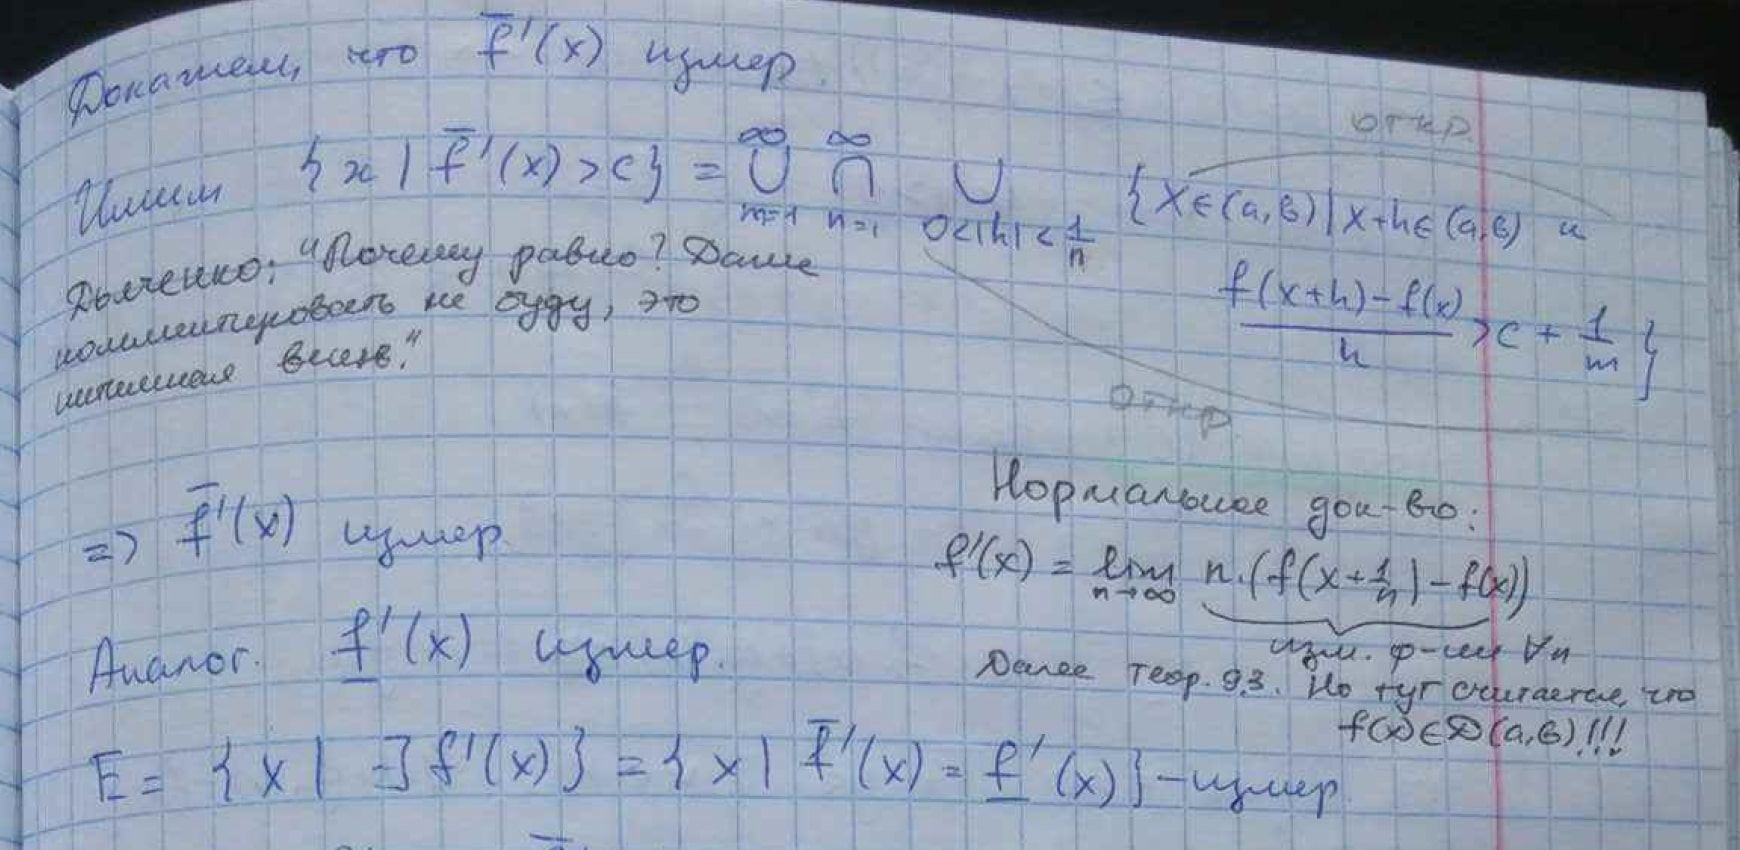
\includegraphics[width=0.8\textwidth]{sets_from_real_calculus.jpg} % замените на своё имя файла
\caption{Пример страшного равенства множеств из лекций по действительному анализу М.И. Дьяченко}
\label{fig:mylabel}
\end{figure}

\subsection*{Отображения множеств}\addcontentsline{toc}{subsection}{Отображения множеств}
\df Отображением $F$ множества $X$ в множество $Y$  (mapping) называется сопоставление каждому элементу $x \in X$ некоторого элемента $y \in Y$. Тогда пишут, что $y = F(x)$, а $F : X \rightarrow Y$ (''$F$ действует из $X$ в $Y$''). 

Если хотят полностью описать отображение, то используется обозначение
$$F : \begin{cases}
X \rightarrow Y & \text{(откуда и куда действует)}\\
x \mapsto y = F(x) & \text{(правило действия)}
\end{cases}$$

Понятие отображения обобщает понятие числовой функции, которая является отображением числовой прямой в саму себя ($X = Y = \R$). Например, функция $f(x) = x + 1$ есть отображение
$$
f : \begin{cases}
    \R \rightarrow \R\\
    x \mapsto x + 1 = y
\end{cases}
$$
Заметим, что в данном случае существует обратное отображение 
\[f^{-1}: 
\begin{cases}
     \R \rightarrow \R\\
     y \mapsto y - 1 = x
\end{cases}\]

\

Но если бы мы взяли функцию $f(x) = 0$, отображающую все числа в ноль, то для нее уже не существует обратной, потому что все числа ''склеились'' в одно.

\df Отображение $F : X \rightarrow Y$ называется инъективным, если никакие два различных элемента $x_1, x_2 \in X$ не склеиваются в один элемент $y \in Y$, т.е. $F(x_1) \neq F(x_2)$.

\df Отображение $F : X \rightarrow Y$ называется сюръективным, если каждому элементу $y \in Y$ соответствует хотя бы один элемент $x \in X$.

\df Отображение $F : X \rightarrow Y$ называется взаимно однозначным (или биективным, или обратимым), если оно одновременно и инъективно, и сюръективно.

\threestars

\noindent\textbf{Упражнение.} Построить все возможные отображения $F: X \rightarrow Y$, где
\[ 
\begin{array}{ll}
     1)\quad X = \{x\}, \ Y = \{y\}, &2) \quad X = \{x_1, x_2\}, \ Y = \{y\},\\
     3)\quad X = \{x\}, \ Y = \{y_1, y_2\},  & 4) \quad X = \{x_1, x_2\}, \ Y = \{y_1, y_2\}
\end{array}
\]
и указать, являются ли эти отображения инъективными, сюръективными и биективными.

\noindent\textbf{Вопрос.} Пусть $X$ --- множество всех людей, $Y$ --- все даты рождения (без года), $F$ --- сопоставление человеку даты его рождения. Является ли это отображение инъективным, сюръективным и биективным?

\threestars
Признаться честно, мы дали ''наивное'' определение отображения. И для текущих целей этого достаточно, поэтому следующие несколько абзацев можно пропускать. Здесь мы дадим еще несколько формальных определений, чтобы дать определение отображению на теоретико-множественном языке.

\df Множество вида $\{a,b\}$ называется парой.

\df Множество вида $\{a, \{a,b\}\}$ называется упорядоченной парой и обозначается $(a,b)$, элемент $a$ называется первым, а элемент $b$ --- вторым.

\df Пусть $X,Y$ --- произвольные множества. Множество всех упорядоченных пар $\{(x,y): x \in X, y \in Y\}$ называется прямым произведением $X$ и $Y$ и обозначается $X \times Y$.

\df Пусть $F \subset X \times Y$. Если $\forall (x', y'), (x'', y'') \in F$ выполняется условие \[x' = x'' \Rightarrow y' = y'',\]
(т.е. одному иксу не может соответствовать сразу два игрека), то $F$ называется отображением из $X$ в $Y$.

Множество всех $x$, таких, что $\exists y \in Y: (x,y) \in F$ называется областью определения $F$, обозначается $D_F$.

Множество всех $y$, таких, что $\exists x \in X : (x, y) \in F$ называется образом $F$, обозначается $F(X)$ или $\Ima (F)$ (от слова image).

\begin{exercise}
    Сформулировать определение инъективности, сюръективности и биективности на языке теории множеств.
\end{exercise}

\subsection*{Мощность множества}\addcontentsline{toc}{subsection}{Мощность множества}
В интуитивном понимании мощность множества (cardinality) это количество элементов в нем. Но это понимание годится только если мы имеем дело с множествами из конечного числа элементов. А это очень сильное ограничение, учитывая, что хотя бы числовые множества (начиная с натуральных чисел) уже не конечны. Поэтому приходится копать глубже.

Идея здесь такова. Конечные множества мы и так хорошо понимаем с точки зрения их ''размера'', это нужно сохранить. В иных случаях посчитать количество элементов мы не можем, но зато можем их сравнивать, пусть и не имея конкретного числа, характеризующего количество элементов в нем.

\threestars
Займемся формализацией приведеннной идеи.

\df Пусть $X, Y$ --- множества. Если существует взаимно однозначное отображение $F: X \rightarrow Y$, то говорят, что множества $X$ и $Y$ равномощны (имеют одинаковую мощность). Обозначается $|X| = |Y|$.

\df Если $X$ равномощно множеству $\{1, 2, \ldots, n\}$, то $X$ называется $n$-элементным, а $n$ называется количеством элементов в $X$. Обозначается $|X| = n$  (иногда $card(X)$).

\df Количество элементов в $\varnothing$ называется ноль и обозначается $0$.

\df Пустое множество и $n$-элементное называются конечными множествами (пишут $|X| < \infty$). Если множество не является конечным, то оно называется бесконечным.

\df Если $X$ равномощно $\mathbb{N}$, то $X$ называется счетным множеством.

\threestars

Хорошо, есть конечные множества, есть бесконечные. В бесконечных мы выделили счетные. А есть ли бесконечные, но не счетные? Можно показать, что $\mathbb{N}$, $\mathbb{Z}$, $\mathbb{Q}$ --- счетные множества, но $\R$ --- несчетно. Причем $\R$ равномощно отрезку $[0,1]$. Множества, равномощные $[0,1]$, называются множествами мощности континуум.

А вот есть ли среди бесконечных множества, имеющие не счетную и не континуумную мощность --- хороший вопрос. Если интересна эта тема, стоит почитать про \href{https://ru.wikipedia.org/wiki/%D0%9A%D0%BE%D0%BD%D1%82%D0%B8%D0%BD%D1%83%D1%83%D0%BC-%D0%B3%D0%B8%D0%BF%D0%BE%D1%82%D0%B5%D0%B7%D0%B0}{континуум-гипотезу}.

\threestars

\noindent\textbf{Упражнение.} Является ли множество $\{\{\varnothing\}\}$ одноэлементным?

\noindent\textbf{Упражнение.} Сколько элементов содержат следующие множества?
\[
\begin{array}{lll}
    1) \quad \{1, 2, 1\}; & 2) \quad \{1, 2, \{1, 2\}\}; & 3) \quad  \{\{2\}\}; \\
    4) \quad \{\{1\}, 1\}; & 5) \quad \{1, \varnothing\}; & 6)\quad \{\{\varnothing\}, \varnothing\}; \\
    7) \quad \{\{\varnothing\}, \{\varnothing\}\}; & 8) \quad \{x, 3x-1\}, \text{ где } x \in \R.
\end{array}
\]

\noindent\textbf{Упражнение.} Найти мощность множества всех подмножеств данного множества $X$, если $|X| = N$.

\noindent\textbf{Упражнение.} Найти мощность множества всех отображений $X \rightarrow Y$, если $|X| = N$, $|Y| = M$.

% \noindent\textbf{Упражнение.} Найти мощность а) множеств из 2 букв алфавита русского языка, среди которых ровно одна гласная (гласными считаем А, Е, Ё, И, О, У, Ы, Э, Ю, Я), б) множества всех подмножеств алфавита русского языка.

\threestars

Подробнее про теорию множеств можно почитать в книге \cite{Viro}, более продвинуто --- в книге Верещагина и Шеня \cite{VereschaginShenSetTheory} или еще подробнее в книге Куратовского и Мостовского \cite{KuratovskijMostovskij1970}.

\section*{Вероятностное пространство}\addcontentsline{toc}{section}{Вероятностное пространство}
\subsection*{Мотивировка}\addcontentsline{toc}{subsection}{Мотивировка}
Представим себя в роли исследователя какого-то явления, вообще говоря, неважно какой природы. Например, в роли физика-экспериментатора. Задача заключается в том, чтобы понять, каким будет результат эксперимента. В некоторых случаях у нас есть достаточно инструментов для того, чтобы точно указать ответ. То есть результат можно предсказать достоверно. Конечно, всегда может упасть луна с неба, и наш расчет не поможет, но такие погрешности нам скорее всего простят.

Однако не всегда есть достаточно информации, умений, возможностей, чтобы дать достоверный ответ. Тогда можно либо развести руками, либо засучить рукава и искать способ получить достоверный ответ, либо попробовать что-то придумать в имеющихся условиях и получить ответ, хоть и не достоверный, но тем не менее полезный.

Тогда разумно возникает идея разделения достоверности на две составляющие: детерминированную (определенную) и случайную (неопределенную). Детерминировано то, что мы знаем о явлении, а случайно то, чего не знаем. Отсюда видно, что разделение это субъективно: у инсайдера гораздо больше информации, чем у обычного трейдера.

А теперь уже и становится ясно, что под вероятностью следует понимать меру того неполного знания, которое имеется у нас об исследуемом явлении.

\threestars

Итак, концепция должна быть ясна, но теперь нужно придать введенным терминам больше точности, чтобы мочь с ними работать. Для этого нужно перевести внимание со случайности на само исследуемое явление, то есть на его свойства. Мы будем предполагать, что нам известны возможные состояния этого явления, иными словами, результаты эксперимента. А различные состояния принимаются с различной степенью достоверности.

Например, мы хотим узнать, какой завтра будет погода. У нас может быть метеостанция, а может не быть, но мы все равно можем с уверенностью сказать, что завтра не будет +50.

Таким образом, неопределенность распределяется между возможными состояниями. Если состояния равнозначны (подбрасывание монетки, подкидывание кости), то по ним распределяется неопределенность в равной степени. Но с прогнозом погоды это уже не так.

\subsection*{Математический подход}\addcontentsline{toc}{subsection}{Математический подход}
\begin{figure}[h] % [h] означает "здесь"
    \centering
    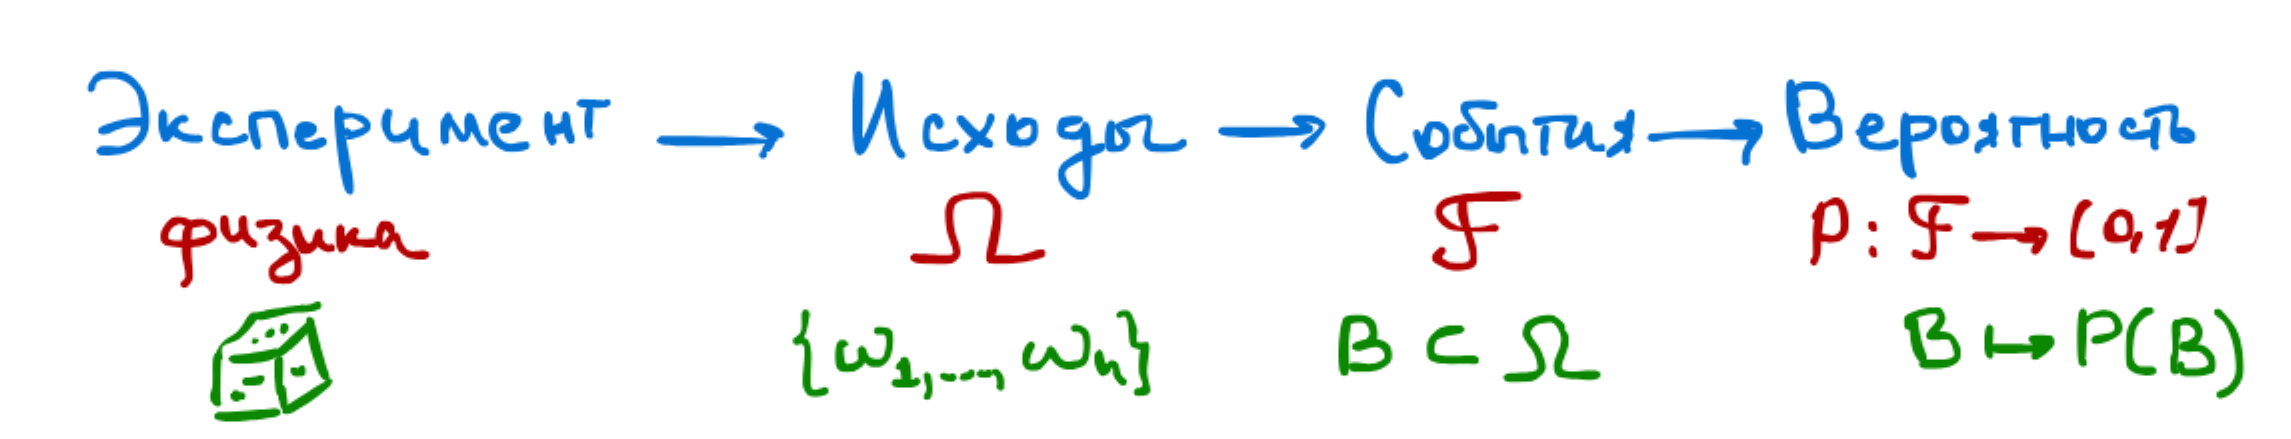
\includegraphics[width=1\textwidth]{scheme_PB_theory} % имя файла без расширения
    \caption{Схема построения вероятностного пространства}
    \label{fig:my_image}
\end{figure}

Здесь мы переведем на язык теории множеств то, о чем было сказано выше. Изложение будет упрощенное, но все равно достаточно нагруженное новой терминологией. Этого хватит для того, чтобы решать задачи с конечным числом исходов и понять основные методы работы с вероятностью.

\df Пространством элементарных исходов (sample space) называется множество, содержащее все возможные взаимоисключающие результаты данного случайного эксперимента, обычно обозначается $\Omega$. Элементы $\Omega$ называются элементарными исходами (outcomes) и обозначаются через $\omega$.

\df Любое подмножество $A \subset \Omega$ называется событием (event). Говорят, что произошло событие $A$, если эксперимент завершился одним из элементарных исходов $\omega \in A$.

\df Пусть $\mathcal{M}$ --- система подмножеств $\Omega$. Функция $m : \mathcal{M} \rightarrow [0, +\infty)$ называется мерой (measure), если $\forall A, B \in \mathcal{M} : A\cap B =  \varnothing$ и $A \cup B \in \mathcal{M}$ верно, что 
$$m(A \cup B) = m(A) + m(B).$$

Если $m(\Omega) = 1$, то мера $m$ называется вероятностной.

\df Тройка $(\Omega, \mathcal{F}, P)$ называется вероятностным пространством (probability space), если $\Omega$ --- пространство элементарных исходов, $\mathcal{F}$ --- множество событий (event space), $P$ --- вероятностная мера на $\mathcal{F}$ (или просто --- вероятность).

При этом система $\mathcal{F}$ должна обладать свойством замкнутости относительно операций объединения и пересечения (объединение/пересечение двух множеств из $\mathcal{F}$ есть множество из $\mathcal{F}$), ведь если мы умеем вычислять вероятность двух событий, то хотим уметь вычислять и вероятность их одновременного выполнения или что хотя бы одно из них выполнилось. Такие системы множеств называются алгебрами.

Задание вероятности $P$ на алгебре $\mathcal{F}$ называется заданием распределения вероятности.

\threestars

Итак, для построения теории вероятностей, мы использовали теорию множеств (чтобы задать исходы $\Omega$ и события $\mathcal{F}$, а также чтобы использовать понятие отображения для задания вероятности $P$), плюс к этому потребовали от $P$ выполнения трех свойств:

\begin{enumerate}
    \item $\forall B \in \mathcal{F} \quad P(B) \ge 0$
    \item $P(A \cup B) = P(A)+P(B)$ для непересекающихся событий $A$ и $B$
    \item $P(\Omega) = 1$
\end{enumerate}

Эти свойства являются аксиомами теории вероятностей. Они были введены А.Н. Колмогоровым в 1933 году в статье, которая в последующем была опубликована на русском языке в \cite{Kolmogorov}.

\begin{figure}[h] % [h] означает "здесь"
    \centering
    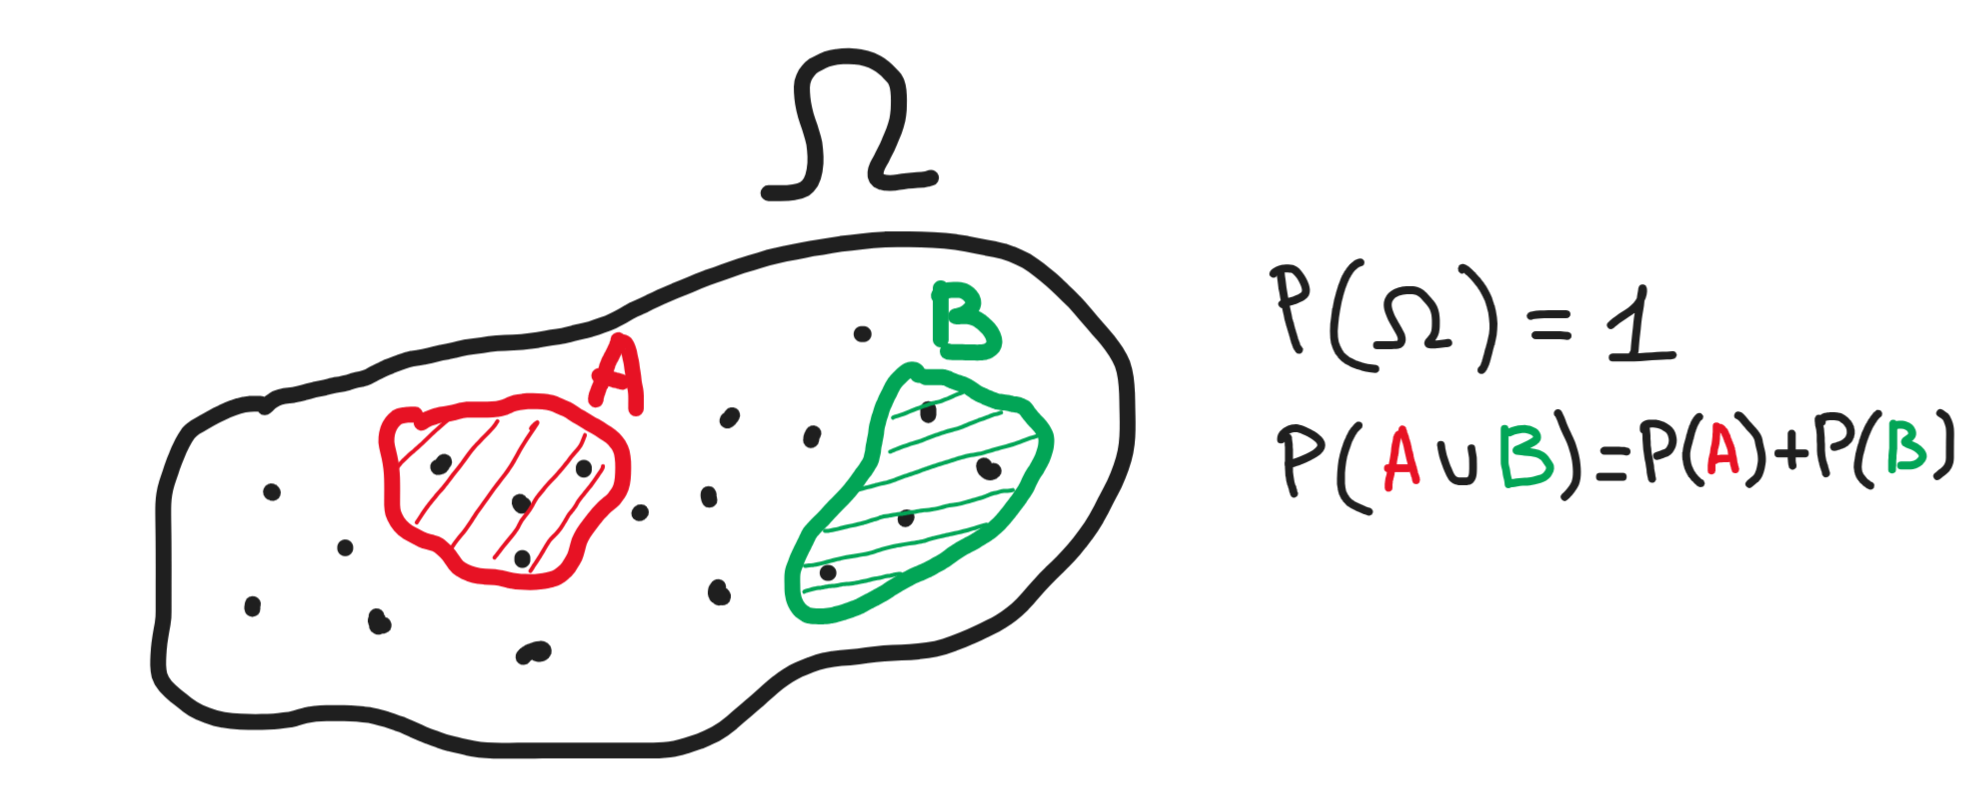
\includegraphics[width=0.7\textwidth]{probability_axioms.png} % имя файла без расширения
    \label{fig:my_image}
\end{figure}

Здесь может быть полезно немного остановиться и подумать, почему именно такие условия наложены на вероятность.

Первое условие объясняется тем, что мы хотим, чтобы наименьшее, что мы можем отмерить есть ничего, то есть ноль. Чуть ниже мы покажем, что мера пустого множества всегда будет нулевой в рамках данного определения. Отмерить множество, которое будет меньше пустого, нельзя.

Второе условие тоже понятно: оно показывает, что мы хотим уметь вычислять вероятности ''сложных'' событий, полученных из простых теоретико-множественными операциями, причем вполне естественным образом: мера объединения непересекающихся множеств равна сумме их мер.

Третье условие утверждает, что событие, состоящее в том, что произойдет хоть что-то, является достоверным. Достоверности приписывается число 1, хотя, конечно, это не принципиально с математической точки зрения. Важно тут то, что эта аксиома специфична именно для теории вероятностей, потому что она по сути реализует концепцию ''достоверности''.

Вообще хотелось бы заметить, что на этой паре страниц произошла магия. Мы совершенно простыми --- как философски, так и математически --- рассуждениями сумели перевести в мир чисел то, что, если вдуматься, бесконечно от них далеко. И дальше из этих трех аксиом вытекает огромная чисто математическая теория.

Обратим еще внимание, что в аксиомах нет никакого намека на связь вероятности с частотностью. Эту связь надо доказывать, и делается это нетривиально. Теорема об этом называется Законом больших чисел.

\threestars
Несколько слов об обозначениях.

Когда рассматривается вероятностное пространство с конечным числом исходов, алгебра событий $\mathcal{F}$ обычно определяется как множество всех подмножеств $\Omega$. Обозначается это так: $\mathcal{F} = 2^\Omega$.

Также, для краткости, часто опускают фигурные скобки под знаком $P(\cdot)$, например, вместо $P(\{\omega\})$ пишут $P(\omega)$. Строго говоря, это неграмотно, но подобных общепринятых сокращений будет в дальнейшем немало.

Обозначение $A \sqcup B$ означает, что объединяются непересекающиеся множества, т.е. $A \cap B = \varnothing$.

\threestars

\noindent\textbf{Теорема (свойства вероятности).}
\begin{enumerate}[label=(\arabic*)]
    \item $P(\varnothing) = 0$
    \item $P(\overline{A}) = 1 - P(A)$
    \item $A \subset B \Rightarrow P(A) \le P(B), \ P(B \setminus A) = P(B) - P(A)$
    \item $P(A \cup B) = P(A) + P(B) - P(AB)$
\end{enumerate}
\begin{proof}
    (1) $P(A \sqcup \varnothing) = P(A) = P(A) + P(\varnothing) \Rightarrow P(\varnothing) = 0$.

    (2) $P(\Omega) = P(A) + P(\overline{A}) = 1 \Rightarrow P(\overline{A}) = 1 - P(A)$.

    (3) $P(B) = P(A) + P(B \setminus A) \Rightarrow P(A) \le P(B), \ P(B \setminus A) = P(B) - P(A)$.

    (4) $P(A \cup B) = P(A) + P(B\setminus A)$, а $P(B \setminus A) = P(B) - P(AB)$.
\end{proof}

\ex Подбрасывание монетки. Определим вероятностное пространство:
\begin{align*}   
&\Omega = \{\text{орел, решка}\},\\
&\mathcal{F} = \{\varnothing, \{\text{орел}\}, \{\text{решка}\}, \{\text{орел, решка}\}\},\\
&P(\{\text{орел}\}) = P(\{\text{решка}\}) = 1/2.
\end{align*}

\noindent\textbf{Вопрос.} Почему именно 1/2? Можно ли задать $P$ как-нибудь иначе?

\subsection*{Как задать вероятность $P$?}\addcontentsline{toc}{subsection}{Как задать вероятность $P$?}
На одном и том же прострастве исходов, вероятность $P$ можно задать различными способами, главное только, чтобы выполнялись аксиомы. Практически, то, как задано распределение, влияет на точность вероятностной модели относительно реального эксперимента. Но пока что мы посмотрим на этот вопрос с чисто теоретической точки зрения.

Допустим, мы как-то хотим задать распределение на $\Omega$, где $|\Omega| = n$. Тогда, формально, надо определить $P$ на всех $2^n$ подмножествах $\Omega$. Но на самом деле эту задачу можно значительно упростить.

Пусть $\Omega = \{\omega_1, \ldots, \omega_n \}$, $\mathcal{F} = 2^\Omega$. Тогда вероятность достаточно задать на каждом из элементарных исходов $P(\omega_i) = p_i$, а не на всем $\mathcal{F}$. Действительно, любое событие $A \in \mathcal{F}$ можно представить как объединение одноэлементных множеств, состоящих из элементарных исходов $\omega_{i_1}, \ldots, \omega_{i_k}$ и тогда, по определению меры, 
$$P(A) = \sum_{j = 1}^kP(\omega_{i_j}) = \sum_{j=1}^k p_{i_j}.$$

\begin{figure}[h] % [h] означает "здесь"
    \centering
    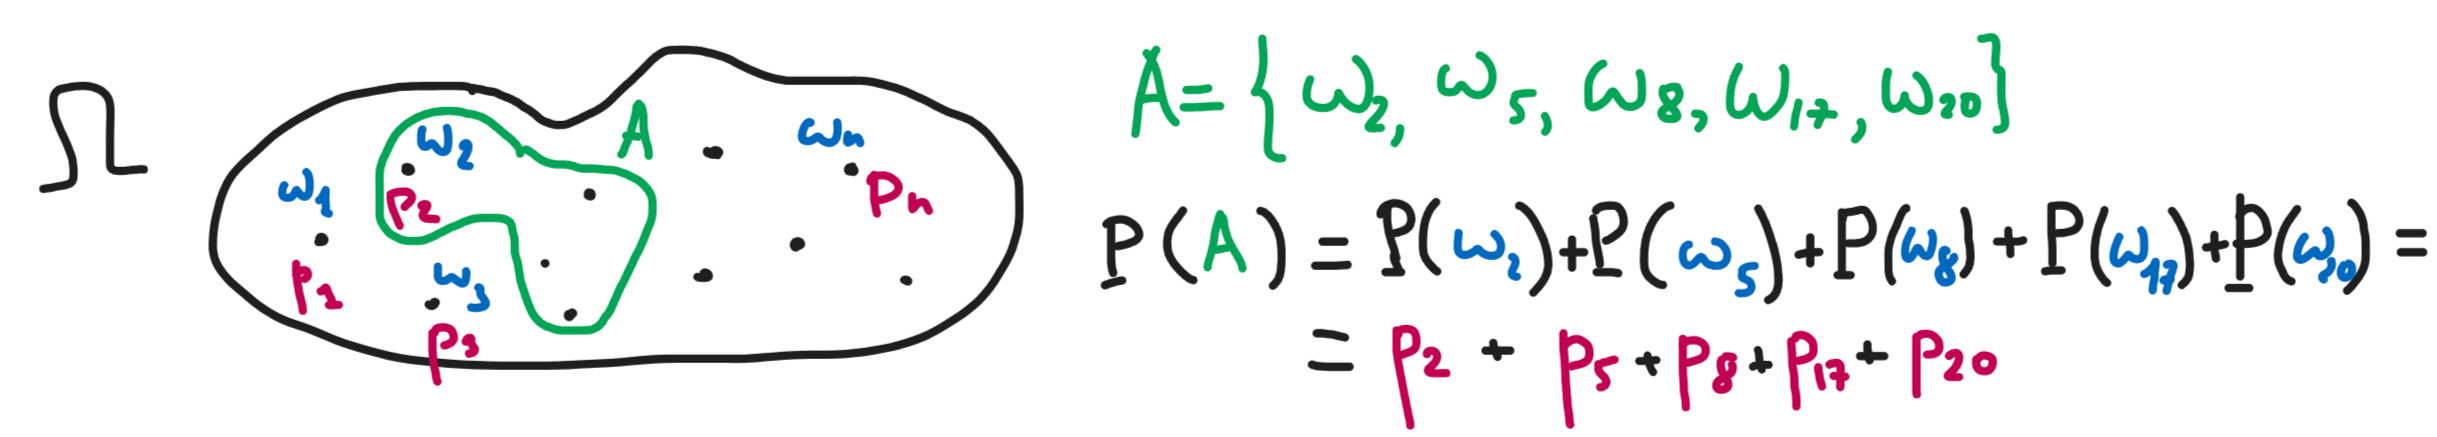
\includegraphics[width=0.9\textwidth]{classic_probability.png} % имя файла без расширения
    \label{fig:my_image}
\end{figure}

\subsection*{Классическое распределение}\addcontentsline{toc}{subsection}{Классическое распределение}

\df Если $|\Omega| = N$ и все $p_i = \frac{1}{N}$, то такое распределение называется классическим.

Классическое распределение соответствует эксперименту, в котором все элементарные исходы равновероятны: монетка считается абсолютно симметричной, кубик обладает идеальной формой, шары в урне неразличимы на ощупь и идеально перемешаны, карты в колоде равномерно перетасованы и т.д.

Понятно, что такие случаи, во-первых, в жизни в чистом виде не встречаются вообще, во-вторых, даже если простить монетке ее неидеальность, все равно классическое распределение покрывает лишь малую часть возможных экспериментов. Но слона нужно есть по кусочкам, поэтому мы и порешаем некоторые задачи на классическую вероятность. Не зря же она классическая.

Заметим только, что классическая вероятность приводит к школьной формуле вычисления вероятности события $A$:
$$\boxed{P(A) = \frac{|A|}{|\Omega|} = \frac{\text{число благоприятных исходов}}{\text{число всех исходов}}}$$

\threestars

Рассмотрим несколько поучительных примеров, показывающих тонкости работы с вероятностными пространствами с равновозможными исходами.

\ex Шестигранный кубик имеет две красные стороны, три зеленых, одну белую. Эксперимент такой: бросаем кубик, смотрим, какой выпал цвет.

\begin{proof}
    Построим вероятностное пространство:
    \[
    \Omega = \{ \text{Красный}, \text{Зеленый}, \text{Белый}\}, \quad \mathcal{F} = 2^\Omega.
    \]
    Можно ли задать вероятность, как
    \[
    P(\{\text{Красный}\}) = P(\{\text{Зеленый}\}) = P(\{\text{Белый}\}) = 1/3 ?
    \]
    Математически --- да, это никак не противоречит аксиомам. Однако, в этом случае выпадения разных граней кубика не будут равновозможными. Поэтому, если мы исходим из предположения о равновозможности выпадения граней кубика, то разумно распределить вероятности так:
    \[
    P(\{\text{Красный}\}) = 2/6, \quad P(\{\text{Зеленый}\}) = 3/6, \quad P(\{\text{Белый}\}) = 1/6.
    \]
\end{proof}

\ex Два игрока подбрасывают монетку. Тот, кто первый победит 6 раз, тот побеждает. Игроков прервали на счете $5:3$. Нужно разделить выигрыш. Как это сделать?

\begin{proof}
Выпишем возможные продолжения игры:
\begin{figure}[h] % [h] означает "здесь"
    \centering
    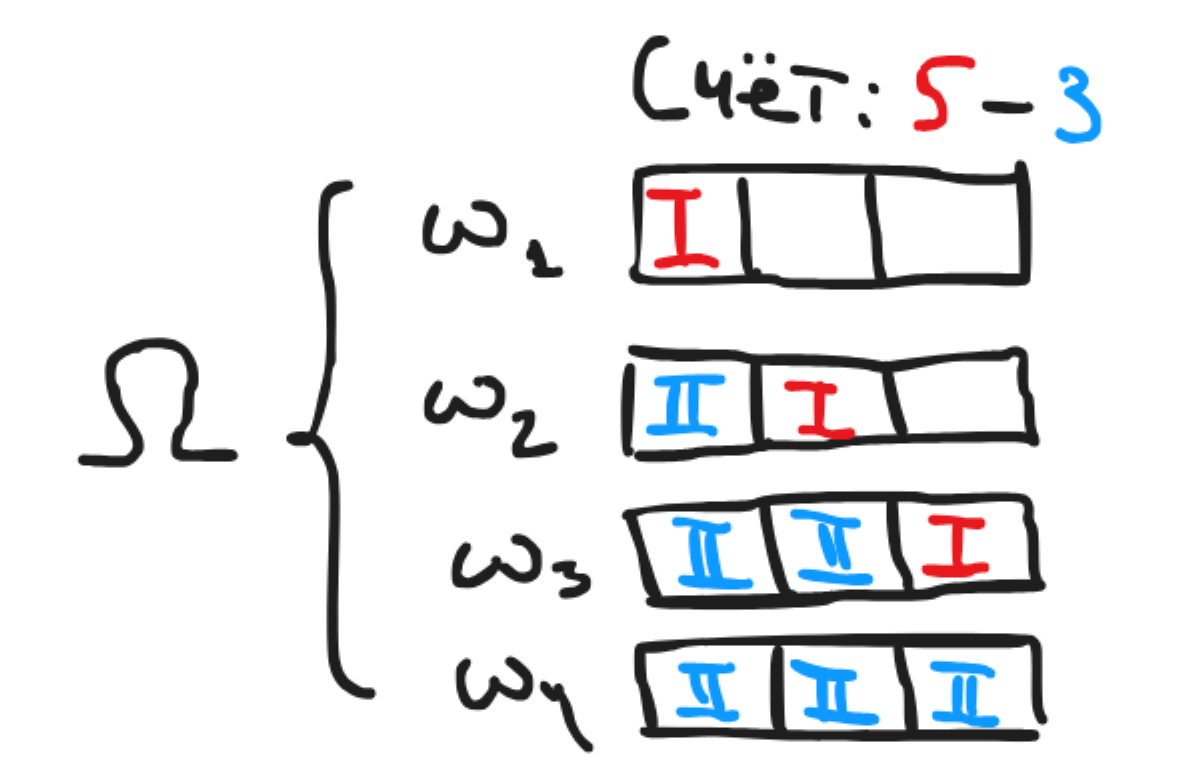
\includegraphics[width=0.4\textwidth]{example_2} % имя файла без расширения
\end{figure}

То есть в трех случаях из четырех побеждает первый игрок. Тогда, если рассматривать $\Omega$ как множество продолжений игры, то можно сделать вывод, что первый победит с вероятностью $3/4$.

Но в этом случае мы почему-то использовали то, что исходы равновероятны. С математической точки зрения, вероятность, определенная таким образом, вполне допустима. Однако, такое распределение не является разумным, так как, физически, равновероятными правильнее считать тройки подбрасываний монеты.

Тогда, первому исходу соответствует сразу четыре тройки, второму исходу --- две, третьему --- одна, четвертому --- одна. И тогда,
\[
P(\omega_1) = 4/8, \quad P(\omega_2) = 2/8, \quad P(\omega_3) = 1/8, \quad P(\omega_4) = 1/8.
\]
А вероятность выигрыша первого игрока равна
\[
P(\{\omega_1, \omega_2, \omega_3\}) = 7/8.
\]
\end{proof}

\ex[\href{https://w.wiki/F2GW}{Задача Банаха о спичках}] Есть два коробка спичек по $n$ штук. Какова вероятность, что первый раз вынув пустой коробок, во втором кармане будет $k$ спичек?

\begin{proof}
    Итак, сначала нужно задать вероятностное пространство, соответствующее условию.

    В качестве равновозможных исходов определим последовательности попыток вытащить спичку из правого или левого кармана. Максимальная длина такой последовательности равна $2n+1$, поэтому
    \[
    \Omega = \{ (a_1, \ldots, a_{2n+1}) : a_i \in \{ \text{П, Л}\} \}
    \]
    Тогда $|\Omega| = 2^{2n+1}$, а вероятность любого исхода --- $1/2^{2n+1}$. Теперь надо посчитать, сколько исходов будут удовлетворять заданному событию.

    Предположим сначала, что пустым оказался коробок из левого кармана, а в правом при этом осталось $k$. Это означает, что к этому моменту были вынуты $n$ левых спичек и $n-k$ правых.

    \begin{figure}[h] % [h] означает "здесь"
        \centering
        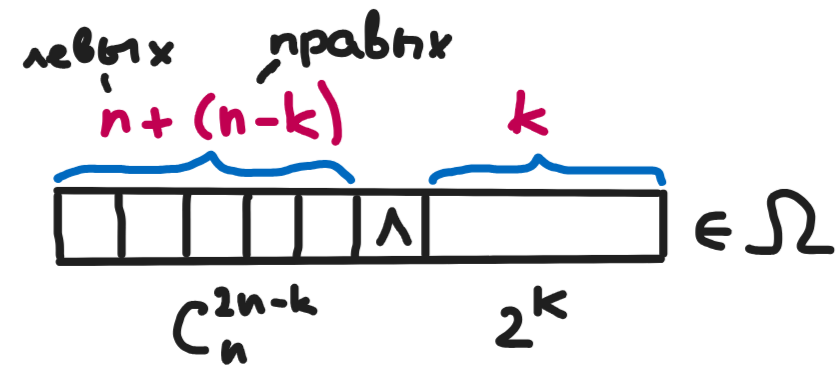
\includegraphics[width=0.4\textwidth]{banach_task.png} % имя файла без расширения
    \end{figure}

    То есть уже достали $n + (n-k) = 2n-k$ спичек, из которых $n$ левых, затем попытались достать спичку из левого кармана, а потом осталось $k$ раз достать оставшиеся спички из правого. Однако, эти $k$ раз не равновозможны, им соответствует $2^k$ исходов из $\Omega$.

    Сколько же комбинаций $(a_1, \ldots, a_{2n-1})$, среди которых $n$ штук $\text{Л}$ и $n-k$ штук $\text{П}$? Расставить $n$ штук $\text{Л}$ по $2n-k$ местам это все равно что достать из $2n-k$ предметов $n$ предметов с номерами этих мест. То есть $C_{2n-k}^n$. Подробнее см. ниже задачи о шарах.

    Таким образом, количество исходов, соответствующих событию, что коробок в левом кармане оказался пуст, а в правом при этом осталось $k$ спичек, равно
    \[
    C_{2n-k}^n \cdot 2^k.
    \]
    Для симметричной ситуации, когда правый коробок оказался пустым, а в левом осталось $k$ спичек, ответ тот же. Поэтому всего исходов, удовляетворяющих заданному событию,
    \[
    2 \cdot C_{2n-k}^{n} \cdot 2^k = 2^{k+1} C_{2n-k}^n.
    \]
    Таким образом, ответ будет такой:
    \[
    \frac{2^{k+1} C_{2n-k}^n}{2^{2n+1}} = \frac{C_{2n-k}^n}{2^{2n-k}}.
    \]
\end{proof}

\subsection*{Четыре задачи о шарах}\addcontentsline{toc}{subsection}{Четыре задачи о шарах}
Знание основ комбинаторики необходимо как для решения самых простых задач на нахождение вероятностей, так и просто для понимания построения математической теории вероятностей. Но, конечно, комбинаторика не привязана именно к вероятности, она существует вполне самодостаточно и пригождается во многих задачах.

Итак, перейдем к модельной задаче, которая в себе содержит вопросы, на которые нам надо получить ответы. Представим, что имеется урна с шарами в размере $N$ штук, и человеку требуется достать из урны $k$ шаров. Вопрос в том, какова вероятность каждого варианта.

\begin{figure}[h] % [h] означает "здесь"
    \centering
    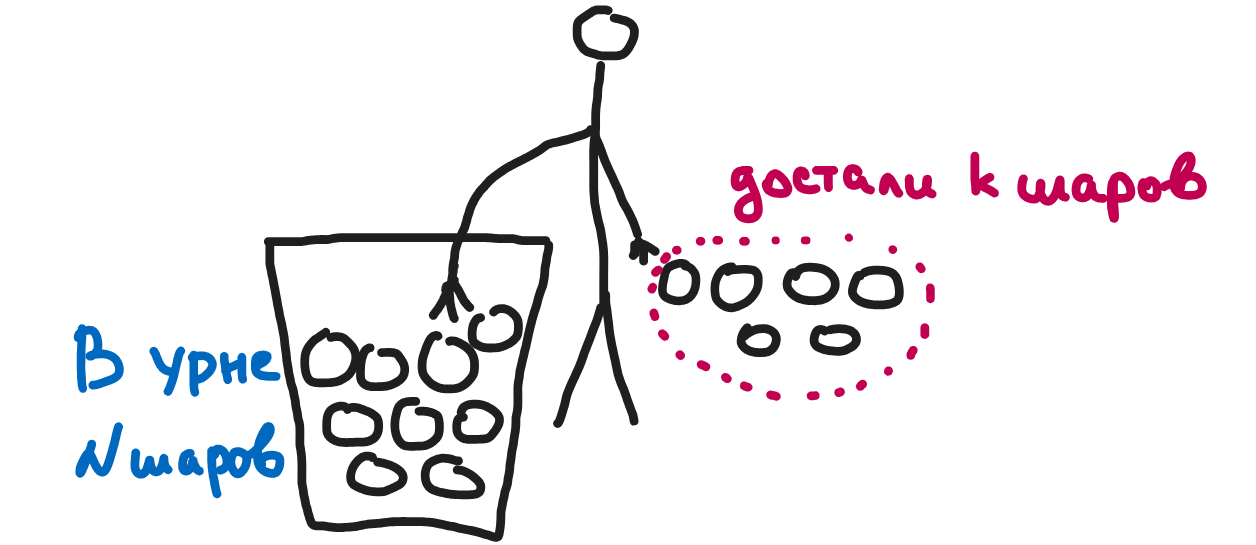
\includegraphics[width=0.7\textwidth]{balls_picture.png}
\end{figure}

Но в формулировке задачи есть нюанс. Мы еще не уточнили, как именно проводится эксперимент, различаются ли как-либо шары в урне, и возвращает ли человек шар после того, как его достал. Отсюда возникает четыре различных случая, которые мы и рассмотрим далее.

\textbf{Задача 1. Упорядоченный выбор с возвращением.}
\begin{proof}
    Строим вероятностное пространство.
    $$\Omega_1 = \{ (i_1, \ldots, i_k) : 1 \le i_s \le N \}, \quad \mathcal{F}_1 = 2^{\Omega_1}.$$
    Мощность $|\Omega_1| = N \cdot \ldots \cdot N = N^k$.\\
    \begin{figure}[h] % [h] означает "здесь"
        \centering
        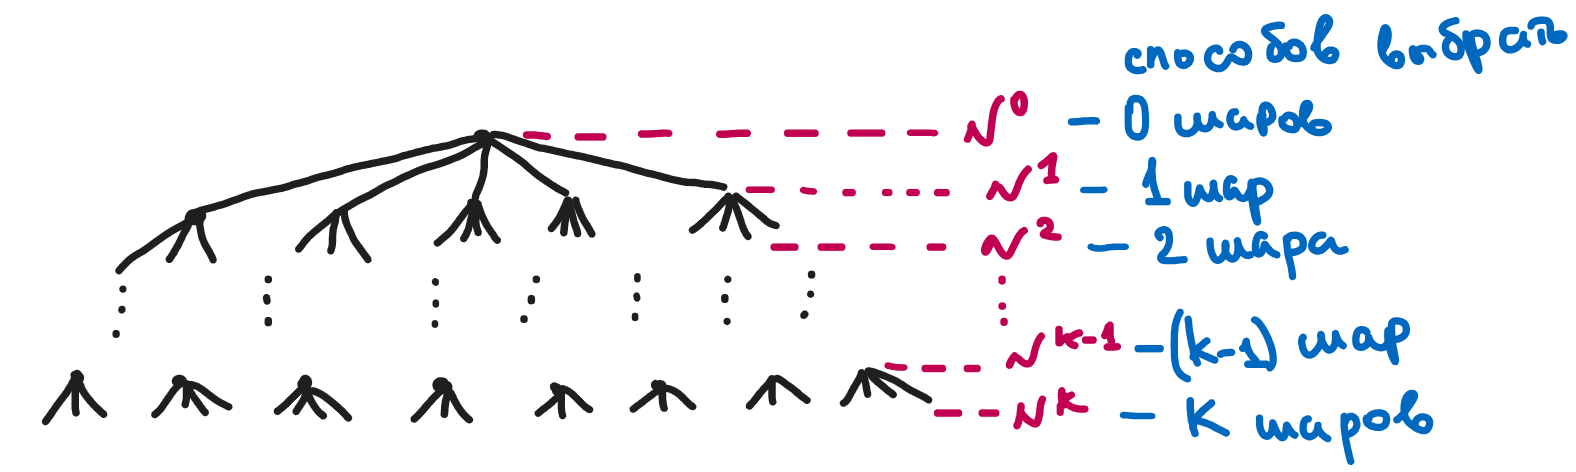
\includegraphics[width=0.7\textwidth]{take_k_balls.png}
    \end{figure}
    
    Число благоприятных исходов (когда вытащили набор $(i_1, \ldots, i_k)$) --- один. Поэтому 
    $$P_1(((i_1, \ldots, i_k)) = \frac{1}{N^k}.$$
    Вероятностное пространство $(\Omega_1, \mathcal{F}_1, P_1)$ задано.
\end{proof}

\textbf{Задача 2. Упорядоченный выбор без возвращения.}
\begin{proof}
    Действуем аналогично.
    $$\Omega_2 = \{ (i_1, \ldots, i_k) : 1 \le i_s \le N, \ i_j \neq i_l \}, \quad \mathcal{F}_2 = 2^{\Omega_2}.$$
    Мощность $|\Omega_2| = N \cdot (N-1) \cdot (N-2)\ldots \cdot (N-k+1) = \frac{N!}{(N-k)!} = A_n^k$.\\
    Число благоприятных исходов (когда вытащили набор $(i_1, \ldots, i_k)$) --- опять один. Поэтому 
    $$P_2(((i_1, \ldots, i_k)) = \frac{1}{A_n^k}.$$
    Вероятностное пространство $(\Omega_2, \mathcal{F}_2, P_2)$ задано.
\end{proof}

\textbf{Задача 3. Неупорядоченный выбор без возвращения.}
\begin{proof}
    Действуем аналогично.
    $$\Omega_3 = \{ \{i_1, \ldots, i_k\} : 1 \le i_s \le N, \ i_j \neq i_l \}, \quad \mathcal{F}_3 = 2^{\Omega_3}$$
    Мощность $|\Omega_3| = \frac{A_n^k}{k!} = \frac{N!}{k! (N-k)!} = C_N^k$.\\
    Число благоприятных исходов (когда вытащили набор $(i_1, \ldots, i_k)$) --- опять один. Поэтому 
    $$P_3(((i_1, \ldots, i_k)) = \frac{1}{C_n^k}$$
    Вероятностное пространство $(\Omega_3, \mathcal{F}_3, P_3)$ задано.
\end{proof}

\textbf{Следствие.} Так как сумма вероятностей элементарных исходов должна равняться единице, то мы получаем формулу
$$\sum_{k=0}^N \frac{1}{C_n^k} = \sum_{k=0}^N \frac{1}{A_n^k}= 1.$$

\textbf{Замечание.} Неупорядоченный выбор без возвращения $k$ шаров из $n$ шаров это то же самое, что расставить $k$ шаров по $n$ ячейкам с номерами, которые заранее подписаны на вытащенных шарах. Поэтому количество способов расставить $k$ одинаковых предметов по $n$ местам --- тоже $C_n^k$.

\textbf{Задача 4. Неупорядоченный выбор с возвращением.}
\begin{proof}
    Здесь пойдем несколько другим путем. Будем представлять исходы в виде вектора чисел, характеризующих, сколько шаров какого типа (сколько первых шаров, сколько вторых и т.д.) в данном наборе шаров.
    $$\Omega_4 = \{ (i_1, \ldots, i_N) : 0 \le i_j \le k, \ i_1 + \cdots + i_N = k \}, \quad \mathcal{F} = 2^{\Omega_4}.$$

    Кстати, линейные уравнения с целыми коэффициентами с поиском решений в целых числах называются диофантовыми. Таким является и наше получившееся уравнение
    \[
    x_1 + \cdots + x_N = k.
    \]
    
    Здесь мы видим, что по сути задача сводится к тому, чтобы посчитать количество разбиений числа $k$ в сумму $N$ чисел от $0$ до $k$.

    Тогда можно представить, как в ряд выложены $k$ шаров, а между ними расположены $N-1$ перегородка, каждая из которых отделяет $i_j$ белых шаров. Но представим еще, что эти перегородки --- тоже шары, допустим черные.

    Таким образом, каждому нашему исходу можно однозначно сопоставить такой набор из белых и черных шаров, выложенных в ряд. То есть способов получить нужное разбиение ровно столько же, сколько есть способов расставить $N-1$ черный шар между $k$ белыми.

    Сколько же способов это сделать? Столько же, сколько способов достать $N-1$ шар из урны с $N+k-1$ одинаковыми шарами. Действительно, представим, что у нас выложено $N+k-1$ белых шаров в ряд, и все они занумернованы. Теперь сваливаем все шары в урну, перемешиваем, достаем $N-1$ шар и красим в черный. Затем достаем все остальные белые шары и выкладываем все шары в порядке подписаных заранее номеров. Получаем некоторое разбиение.

    \begin{figure}[h] % [h] означает "здесь"
        \centering
        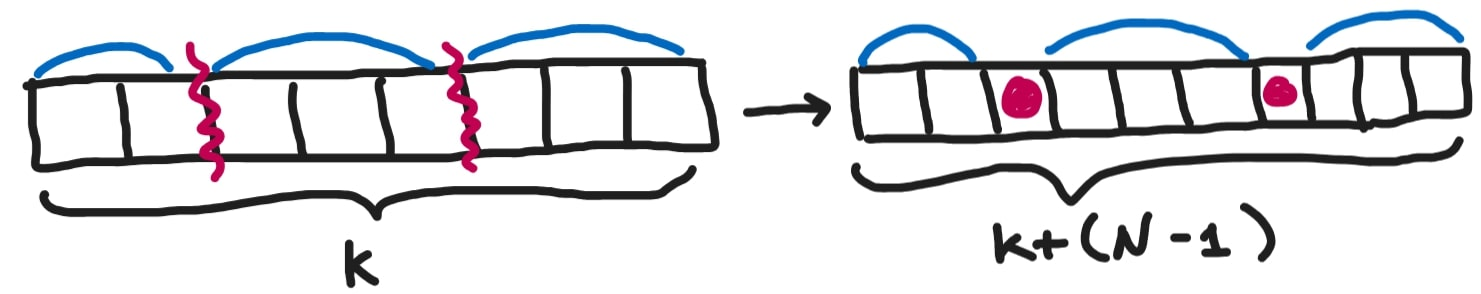
\includegraphics[width=0.7\textwidth]{pictures/fourth_problem_about_balls.jpg}
    \end{figure}

    Итак, любое разбиение вида $k = i_1 + \cdots + i_N$ означает, что из урны с $N+k-1$ шарами достали и перекрасили в черный шары с номерами $i_1+1, i_2+i_1+1, \ldots, i_N+\cdots+i_1+1$. То есть число разбиений равно числу способов достать $N-1$ шар из урны с $N+k-1$ шарами, а это число, по задаче 3, равно $C_{N-k+1}^{N-1}$.

    Значит, мощность $|\Omega_4| = C_{N-k+1}^{N-1}$.\\
    Поэтому 
    $$P(((i_1, \ldots, i_k)) = \frac{1}{C_{N-k+1}^{N-1}}.$$
    Вероятностое пространство $(\Omega_4, \mathcal{F}_4, P_4)$ задано.
\end{proof}

\textbf{Упражнение*.} Как еще можно построить вероятностное пространство в задаче 4?

\task[1] Сколько подмножеств у $n$-элементного множества? (Указание: использовать первую задачу о шарах).

\task[2] а) Сколько $m$-элементных подмножеств у $n$-элементного множества? б) Доказать, что
\[
\sum_{k=0}^n C_n^k = 2^n.
\]

\task[3] а) Сколько встреч будет проведено в турнире 20 команд по круговой системе (в 1 круг)?

б) Сколькими способами можно собрать команду программистов из $5$ человек, когда имеется $30$ программистов?

\task[4] Сколькими способами можно разделить десять задач в Jira по пяти программистам? (Указание: применить идею из четвертой задачи о шарах).

\task[5] Доказать, что
\[
C_n^k = C_n^{n-k}
\]
используя и не используя прямой подсчет. Отсюда вытекает симметричность треугольника Паскаля.

\task[6] Доказать реккуррентную формулу (треугольник Паскаля)
\[
C_n^k = C_{n-1}^{k-1} + C_{n-1}^k
\]
используя и не используя прямой подсчет.

\subsection*{Еще задачи}\addcontentsline{toc}{subsection}{Еще задачи}

\task[1.1 из \cite{ZubkovSevostyanovChistyakov1989}] Из ящика, содержащего три билета с номерами 1, 2, 3, вынимают по одному все билеты. Предполагается, что все последовательности номеров билетов имеют одинаковые вероятности. Найти вероятность того, что хотя бы у одного билета порядковый номер совпадает с собственным.

\begin{proof}
    Определим вероятностое пространство:
    \begin{align*}
        &\Omega = \{ (a,b,c) : a, b, c \in \{1,2,3\} \text{ -- различны} \}\\
        &\mathcal{F} = 2^\Omega\\
        &P((a,b,c)) = \frac{1}{|\Omega|} = \frac{1}{6}
    \end{align*}
    Выпишем все варианты последовательностей:
    \begin{align*}
        &(1, 2, 3)\\
        &(1, 3, 2)\\
        &(2, 1, 3)\\
        &(2, 3, 1)\\
        &(3, 1, 2)\\
        &(3, 2, 1)
    \end{align*}
    Видим, что подходящих вариантов четыре, значит, ответ $4/6 = 2/3$.
\end{proof}

\task[1.2 из \cite{ZubkovSevostyanovChistyakov1989}] Колода из 36 карт хорошо перемешана (т.е. все возможные расположения карт равновероятны). Найти вероятности событий
\[
\begin{aligned}
A &= \{ \, \text{четыре туза расположены рядом} \, \}\\
B &= \{ \, \text{места расположения тузов образуют} \\
  &\hspace{2.0em} \text{арифметическую прогрессию с шагом 7} \, \}
\end{aligned}
\]

\begin{proof}
    Определим вероятностное пространство:
    \begin{align*}
        &\Omega = \{ (i_1, \ldots, i_{36}) : i_j \in \{1, \ldots, 36\} \text{ -- различны} \}\\
        &\mathcal{F} = 2^\Omega\\
        &P((i_1, \ldots, i_{36})) = \frac{1}{|\Omega|} = \frac{1}{36!}
    \end{align*}
    Тогда
    \[
    A = \{ (i_1, \ldots, i_{36}) : \exists j \le 33: i_j, i_{j+1},  i_{j+2}, i_{j+3} - \text{ номера тузов}\}
    \]
    Таким образом, имеем 33 позиции для четверки тузов и еще $4! = 24$ способов их между собой переставить и $32!$ способа переставить оставшиеся карты. Значит, $|A| = 33 \cdot 4! \cdot 32!$.
    \[
    P(A) = \frac{|A|}{|\Omega|} = \frac{33 \cdot 4! \cdot 32!}{36!} = \frac{33 \cdot 24}{33 \cdot 34 \cdot 35 \cdot 36} = \frac{24}{34 \cdot 35 \cdot 36} \approx 0.00056 .
    \]

    Теперь зададим событие $B$:
    \[
    B = \{ (i_1, \ldots, i_{36}) : \exists j \le 15: i_j, i_{j+7}, i_{j+14}, i_{j+21} - \text{номера тузов} \}
    \]
    Значит, можно поставить первый туз на первые $15$ мест, переставлять их между собой и переставлять оставшиеся карты, т.е.
    \[
    |B| = 15 \cdot 4! \cdot 32!
    \]
    Поэтому
    \[
    P(B) = \frac{|B|}{|\Omega|} = \frac{15 \cdot 4! \cdot 32!}{36!} = \frac{15 \cdot 24}{33 \cdot 34\cdot35\cdot 36} \approx 0.0002546 .
    \]
\end{proof}

\task[1 из листка 1 лекций Шапошникова.] $N$ человек принесли подарки друг для друга. Затем этим подарки сложили в мешок и наугад каждый вынул из мешка себе подарок. Какова вероятность того, что конкретный человек вынул подарок, который он принес? Какова вероятность того, что никто не вытащил подарок, который сам принес?

\begin{proof}
    Вероятностное пространство состоит из пространства исходов
    \[
    \Omega = \{ (a_1, \ldots, a_N) : 1 \le a_i \le N, a_i \neq a_j \}
    \]
    с классической вероятностью. Наборы упорядоченные, так как важно кто какой подарок получил.

    Событие $A = \{\text{конкретный человек вынул свой подарок}\}$ имеет мощность
    \[
    |A| = 1 \cdot (N-1) \cdot (N-2) \cdots 2 = (N-1)!,
    \]
    таким образом,
    \[
    P(A) = \frac{|A|}{|\Omega|} = \frac{(N-1)!}{N!} = \frac{1}{N}.
    \]

    Рассмотрим теперь событие $B = \{\text{никто не вытащил свой подарок}\}$. Представим его в виде пересечения событий $B_i = \{\text{i-ый человек вытащил не свой подарок}\}$, тогда
    \[
    B = \bigcap_{i=1}^N B_i.
    \]
    Мощность пересечения считать сложно, а вот мощность объединения можно вычислить с помощью формулы включений-исключений. Поэтому попробуем найти мощность
    \[
    \overline{B} = \overline{\bigcap_{i=1}^N B_i} = \bigcup_{i=1}^N \overline{B_i}.
    \]
    Тогда по формуле включений-исключений имеем
    \[
    |\overline{B}| = \sum_{i=1}^N |\overline{B_i}| - \sum_{i < j} |\overline{B_i} \cap \overline{B_j}| + \sum_{i < j < k} |\overline{B_i} \cap \overline{B_j} \cap \overline{B_k}| + \cdots + (-1)^{N+1} |\overline{B_1} \cap \cdots \cap \overline{B_N}|.
    \]
    Итак, мощность $\overline{B_i}$ мы уже считали (для события $A$), т.е. $|\overline{B_i}| = (N-1)!$. 
    
    Пересечение событий $\overline{B_i}$ означает, что несколько человек взяли свои подарки. Аналогично рассуждая, получаем, что
    \[
    \forall i < j \quad |\overline{B_i} \cap \overline{B_j}| = (N-2)!
    \]
    и так далее для всех пересечений. Значит,
    \begin{align*}
        |\overline{B}| &= \sum_{i=1}^N (N-1)! - \sum_{i < j} (N-2)! + \sum_{i < j < k} (N-3)! + \cdots + (-1)^{N+1} =\\
        & = N(N-1)! - C_N^2 (N-2)! + C_N^3 (N-3)! + \cdots + (-1)^{N+1} = \\
        & = N! - \frac{N!}{2!} + \frac{N!}{3!} - \cdots + (-1)^{N+1}
    \end{align*}
    Значит,
    \begin{align*}
        P(\overline{B}) &= \frac{|\overline{B}|}{|\Omega|} = \frac{N! - \frac{N!}{2!} + \frac{N!}{3!} - \cdots + (-1)^{N+1}}{N!} = \\
        & = 1 - \frac{1}{2!} + \frac{1}{3!} - \cdots + \frac{(-1)^{N+1}}{N!}.
    \end{align*}
    Отсюда
    \[
    P(B) = 1 - P(\overline{B}) = \frac{1}{2!} - \frac{1}{3!} + \cdots + \frac{(-1)^N}{N!}.
    \]
    Но это еще не все. Если знать, что
    \[
    e^x = 1 + x + \frac{x^2}{2!} + \frac{x^3}{3!} +\cdots + \frac{x^k}{k!} + \cdots \approx 1 + x +\frac{x^2}{2!} + \cdots + \frac{x^N}{N!}, \quad N \rightarrow \infty,
    \]
    то, можно заметить, что
    \[
    P(B) \approx e^{-1} \approx 0.368.
    \]
\end{proof}

\task[1 (Задача 2 из \href{https://old.mccme.ru/ium//postscript/s24/ProbTh-list1-24s.pdf}{листка 1 Шапошникова})] Сто мудрецов по одному заходят в комнату, в которой стоят сто закрытых коробок. В каждой коробке лежит табличка с именем одного из мудрецов. Все имена различны. Мудрец открывает 50 коробок одну за другой в произвольном порядке. Если в одной из открытых им коробок есть его имя, то он выживает, а если нет, то погибает. После каждого мудреца все коробки закрывают и оставшиеся мудрецы не знают о судьбе ушедших в комнату. Изначально мудрецы находятся вместе и могут продумать план действий. Придумайте плат, который гарантирует выживание всех мудрецов с вероятностью не менее $1/4$.
\begin{proof}
    
\end{proof}

\task[1.39] Найти вероятность того, что при случайной расстановке двух ладей на шахматной доске они не будут угрожать друг другу.

\task[1.40*] Найти вероятность $P_k$ того, что при случайной расстановке $2 \le k \le 8$ ладей на шахматной доске они не будут угрожать друг другу. При каких $k$ вероятность меньше $1/2$? Меньше $1/1000$?

\section*{Условная вероятность}\addcontentsline{toc}{section}{Условная вероятность}

Мы говорили о том, что вероятность субъективна, то есть зависит от того, какую информацию о физике эксперимента мы имеем. Поэтому важно уметь пересчитывать вероятность события после того, как были получены новые сведения.

Когда игрок в покер читает по лицу оппонента, пришла ли тому хорошая карта или плохая, он получает дополнительную информацию, которая влияет на принятие решения о дальнейших действиях.

Пересчитанную вероятность с учетом новых знаний называют условной, то есть вероятность события при условии, что уже известно что-то еще.

\threestars

\ex Кидается кубик. Какова вероятность, что выпало число меньше или равно трех, если известно, что выпало четное?
\begin{proof}
    Отбрасываем все нечетные исходы, остаются только $2,4,6$. Среди четных подходит только двойка. Значит вероятность равна $1/3$.
\end{proof}

\textbf{Вопрос.} Перед тем, как идти дальше, стоит попробовать сформулировать общее определение условной вероятности в случае равновероятных исходов.

\df Пусть $P(B) > 0$. Тогда вероятностью события $A$ при условии события $B$ (conditional probability) называется число
\[
P(A \mid B) = \frac{P(A \cap B)}{P(B)}.
\]

\begin{figure}[h] % [h] означает "здесь"
    \centering
    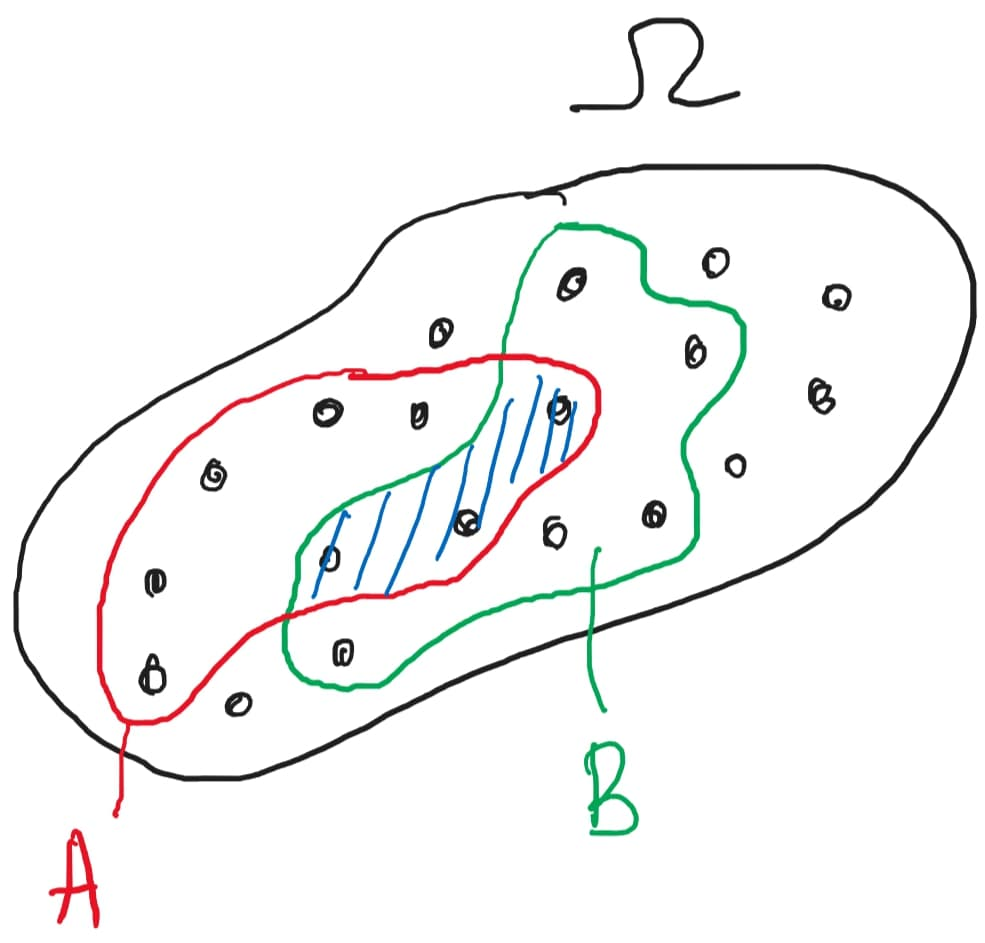
\includegraphics[width=0.3\textwidth]{pictures/cond probability.jpg}
\end{figure}

Почему именно такая формула? Идея в следующем. Изначально было известно, что вероятность как-то распределена по исходам $\Omega$, но когда стало известно $B$, то теперь про распределение стало известно точно, что попасть в $\overline{B}$ вероятность равна нулю. То есть в некотором смысле пространство исходов сузилось, и теперь уже вероятность события $A$ ищется в мире, где исходы извне $B$ невозможны.

Поэтому если вначале вероятностью $A$ мы называли, говоря интуитивным языком, долю знания о $A$ относительно $\Omega$, то теперь, зная, что $B$ произошло, вероятность $A$ это доля знания о нем относительно $B$. Об этом и говорит определение.

\textbf{Утв.} Отображение 
\[
    P_B(\cdot) \equiv P(\  \cdot \mid B) :
\begin{cases}
    2^{\Omega} \rightarrow [0,1]\\
    A \mapsto P(A \mid B)
\end{cases}
\]
является вероятностной мерой на $\Omega$. Причем $P_B(B) = P(B \mid B) = 1$.

\practice Доказать предыдущее утверждение (проверить аксиомы).

\ex В урне 15 белых и 13 черных шаров. Вынимается два шара (упорядоченно без возвращения). Какова вероятность, что оба --- белые?

\begin{proof}
\begin{align*}
    P&(\{\text{оба белые\})} = P(\{\text{первый белый}\} \cap \{\text{второй белый}\}) = \\
    &= P(\{\text{второй белый}\} \mid \{\text{первый белый}\}) P(\{\text{первый белый}\}) = \\
    &=\frac{14}{27} \cdot \frac{15}{28}.
\end{align*}
\end{proof}

\ex Какова вероятность, что второй шар --- белый?

\begin{proof}
    \begin{align*}
        P(\text{2-й белый}) & = P(\text{2-й белый, 1-й белый)} + P(\text{2-й белый, 1-й черный)} = \\
        & = P(\text{2-й белый} \mid \text{1-й белый)} P(\text{1-й белый}) + \\
        & + P(\text{2-й белый} \mid \text{1-й черный)} P(\text{1-й черный}) = \\
        & = \frac{14}{27} \cdot \frac{15}{28} + \frac{15}{27} \cdot \frac{13}{28} = \frac{15}{28}.
    \end{align*}
\end{proof}

\begin{figure}[h] % [h] означает "здесь"
    \centering
    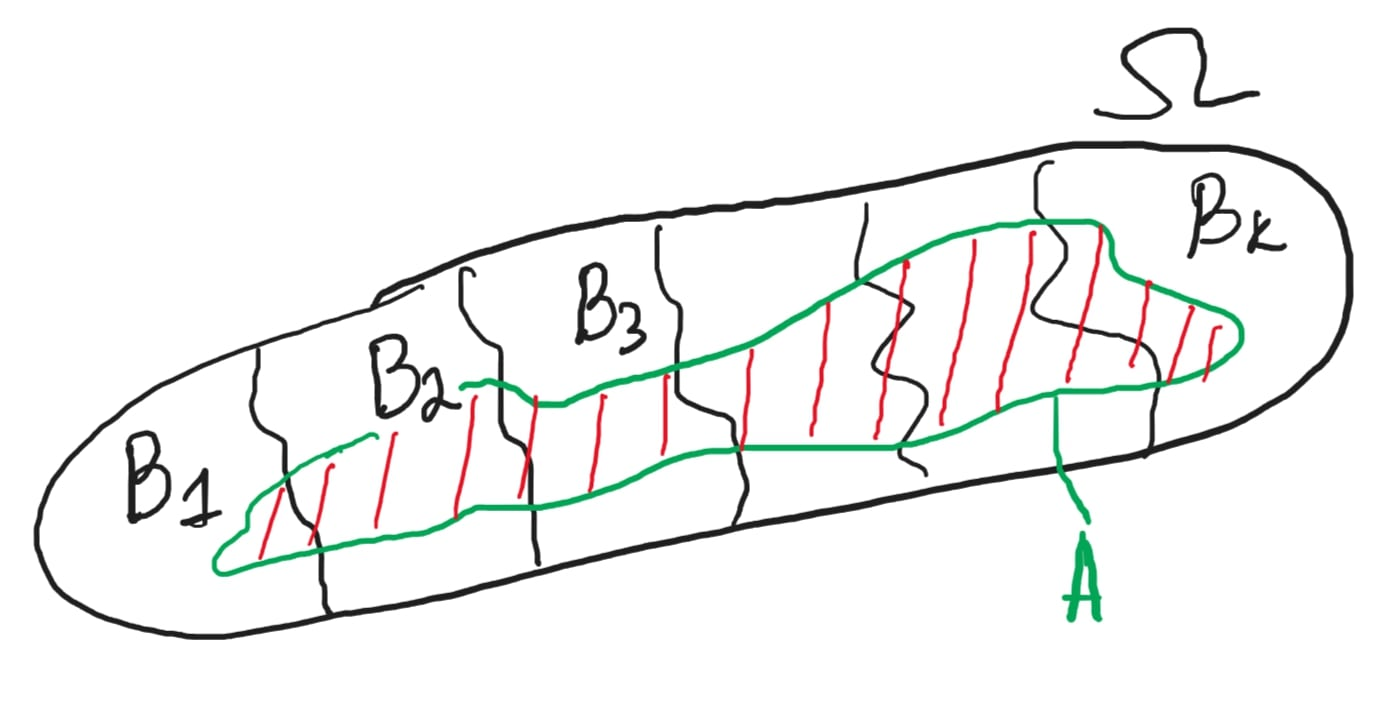
\includegraphics[width=0.5\textwidth]{pictures/total probability.jpg}
\end{figure}

\theor[Формула полной вероятности / Law of Total Probability] Пусть 
$$\Omega = \bigsqcup_{k=1}^n B_k, \quad P(B_k) > 0.$$
Тогда
\[
\forall A \in 2^\Omega \quad P(A) = \sum_{k=1}^n P(A \mid B_k) P(B_k).
\]

\begin{proof}
    Разобьем $A$ на кусочки
    \[
    A = \bigsqcup_{k=1}^n A \cap B_k.
    \]
    Тогда, по аксиоме аддитивности,
    \[
    P(A) = \sum_{k=1}^n P(A \cap B_k).
    \]
    Но по определению условной вероятности
    \[
    P(A \cap B_k) = P(A \mid B_k) P(B_k).
    \]
\end{proof}

\ex Монета лежит орлом вверх, а что с другой стороны --- не знаем (либо тоже орел, либо решка). Бросили монету три раза. Найти вероятность того, что выпадет три раза орел.

\begin{proof}
    Обозначим события
    \begin{align*}
        &B_1 = \{\text{монета с двумя орлами}\}\\
        &B_2 = \{\text{монета с орлом и решкой}\}\\
        &A = \{\text{выпало три орла}\}
    \end{align*}
    Тогда по формуле полной вероятности получаем
    \begin{align*}
        P(A) &= P(A \mid B_1) P(B_1) + P(A \mid B_2)P(B_2) = \\
        & = 1 \cdot \frac{1}{2} + \frac{1}{8} \cdot \frac{1}{2} = \frac{9}{16}.
    \end{align*}
\end{proof}

\ex Какая вероятность того, что монета с двумя орлами, зная, что выпало три орла?

\begin{proof}
    \begin{align*}
        P(B_1 \mid A) &= \frac{P(B_1 A)}{P(A)} = \frac{P(A \mid B_1) P(B_1)}{P(A \mid B_1) P(B_1) + P(A \mid B_2)P(B_2)} = \\
        &= \frac{1 \cdot \frac{1}{2}}{1 \cdot \frac{1}{2} + \frac{1}{8} \cdot \frac{1}{2}} = \frac{8}{9}.
    \end{align*}
\end{proof}

\begin{exercise}
    Что будет, если рассмотреть произвольное число бросков $n$ и устремить его к бесконечности?
\end{exercise} 

\theor[Формула Байеса, Thomas Bayes, 1763]
\[
\Omega = \bigsqcup_{i=1}^n B_i \quad \Rightarrow \quad P(B_j \mid A) = \frac{P(A \mid B_j) P(B_j)}{\sum_{i=1}^n P(A \mid B_i) P(B_i)}.
\]
\begin{proof}
    Очевидно (см. пример выше): комбинация определения и формулы полной вероятности.
\end{proof}

Смысл формулы в том, чтобы связать условные вероятности $P(A \mid B)$ и $P(B \mid A)$. Это удобно, когда условие сложное, а событие простое. Дальше в примерах посмотрим, насколько это мощный инструмент.

\threestars

\ex[Парадокс Байеса] Человек подозревает, что он болен. Имеется тест, который может ошибаться. Обозначим
\begin{align*}
    &B_1 = \{ \text{болен} \}\\
    &B_2 = \{ \text{здоров} \}
\end{align*}
Дано, что $P(B_1) = 0.01$. Также пусть $A = \{\text{тест сказал, что болен}\}$. Известно, что $P(A \mid B_1) = 0.99$, $P(A \mid B_2) = 0.02$. Найти $P(B_1 \mid A)$.

\begin{proof}
    Применим формулу Байеса:
    \[
    P(B_1 \mid A) = \frac{P(A \mid B_1) P(B_1)}{P(A \mid B_1) P(B_1) + P(A \mid B_2) P(B_2)} = \frac{0.99 \cdot 0.01}{0.99 \cdot 0.01 + 0.02 \cdot 0.99} = \frac{1}{3}.
    \]
    Таким образом, если тест сказал, что человек болен, лишь в \textbf{трети} случаев это окажется правдой. Разберемся, в чем тут дело.

    Посмотрим, засчет чего вероятность так мала. Вероятности $P(B_1)$ и $P(B_2)$ относится к природе заболевания, а не к тесту. Вероятность $P(A \mid B_1)$ показывает точность теста, но она и так довольно высока: даже если бы она была равна единице, результат был бы не сильно лучше. А вот $P(A \mid B_2)$, играет ключевую роль: при уменьшении этой вероятности, результат приближается к единице.

    Отсюда можно сделать вывод, что точность теста в случае, если человек здоров, слишком мала для такой распространенности заболевания. Значит ли это, что тест плох? Что было бы лучше взять тест, который просто всегда говорит ''здоров'' и тем самым угадывает с вероятностью 0.99? Не совсем.

    Пусть $C = \{\text{тест показал, что здоров} \}$. Посчитаем теперь вероятность
    \[
    P(B_1 \mid C) = \frac{P(C \mid B_1) P(B_1)}{P(C \mid B_1) P(B_1) + P(C \mid B_2) P(B_2)} = \frac{0.01 \cdot 0.01}{0.01 \cdot 0.01 + 0.98 \cdot 0.99} \approx 10^{-4}.
    \]
    Значит, в случае если тест показал, что человек здоров, то в это можно верить, а если показал, что болен, то нужно продолжить исследование --- скорее всего человек здоров. Пример такого теста --- маммография.
\end{proof}

\begin{figure}[h] % [h] означает "здесь"
    \centering
    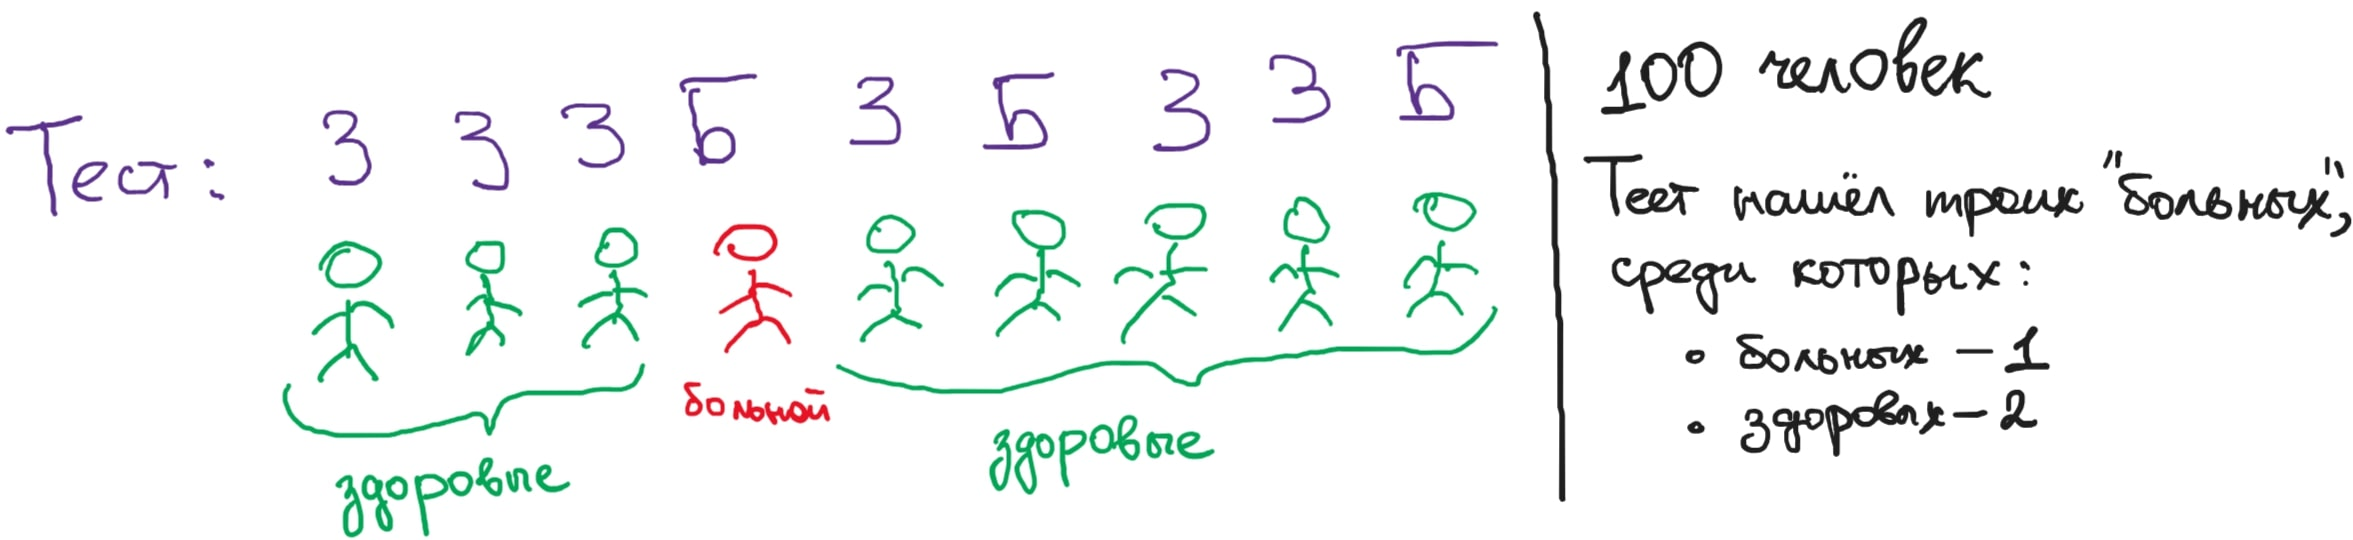
\includegraphics[width=0.9\textwidth]{pictures/test_illness_bayes.jpg}
\end{figure}

\ex[Пародокс Монти--Холла] Перед игроком три двери. За одной из них автомобиль, за двумя другими --- козы. Он выбирает первую дверь, после чего ведущий открывает одну из других дверей, за которой коза. Ведущий предлагает игроку изменить свой выбор. Имеет ли смысл соглашаться?

\begin{proof}
    Интуитивно кажется, что вероятность выигрыша --- $1/2$, так как дверей осталось две, за одной точно автомобиль, а за другой --- коза. Однако, это не так.

    Есть несколько способов решать эту задачу. Мы рассмотрим два. Первый опирается больше на логику и рассуждения, второй использует формулу Байеса.

    \textbf{Решение 1 (логическое).}\\
    Итак, изначально вероятность выигрыша равняется $1/3$, так как автомобиль с равной возможностью находится за одной из трех дверей. Значит вероятность проигрыша, то есть того, что автомобиль находится за второй или третьей дверью, равна $2/3$.

    Далее ведущий открывает третью дверь, за которой находится коза. Значит, вероятность того, что автомобиль за второй дверью теперь равна $2/3$, ведь за третьей дверью коза.

    Поэтому игрок повысит свои шансы на выигрыш в два раза, если поменяет выбор.

    Чтобы лучше прочувствовать, что произошло, можно рассмотреть несколько иную постановку задачи. Предположим, что дверей теперь 100. За одной дверью --- авто. Игрок выбирает первую дверь. Тогда ведущий открывает 98 дверей, за которыми козы. Тот же вопрос, стоит ли игроку изменить выбор на ту дверь, которую ведущий оставил закрытой?

    Становится понятно, что ведущий своим действием дает подсказку (или, скажем точнее, дополнительную информацию) относительно тех дверей, которые не выбраны игроком.

    \textbf{Решение 2 (формула Байеса).}\\
    Если приведенное выше рассуждение не кажется убедительным, то это решение должно все расставить на свои места.

    Итак, чтобы применить формулу Байеса, нужно определить, какие события рассматриваются. Нам надо сравнить вероятности двух событий:
    \begin{itemize}
        \item автомобиль находится за \textbf{первой} дверью при условии, что ведущий открыл третью дверь \textit{после того, как игрок выбрал первую дверь}
        \item автомобиль находится за \textbf{второй} дверью при условии, что ведущий открыл третью дверь \textit{после того, как игрок выбрал первую дверь}
    \end{itemize}

    Найдем вероятность второго события. Из формулировки события сразу напрашиваются обозначения:
    \begin{align*}
        &A_i = \{\text{автомобиль находится за i-ой дверью}\}\\
        &B_i = \{\text{ведущий открыл i-ую дверь после того, как игрок выбрал первую}\}
    \end{align*}
    Тогда требуется найти $P(A_2 \mid B_3)$. Так как события $A_i$ образуют полную систему событий, т.е. $\Omega = A_1 \sqcup A_2 \sqcup A_3$, можно применить формулу Байеса
    \begin{align*}
        P(A_2 \mid B_3) &= \frac{P(B_3 \mid A_2) P(A_2)}{P(B_3 \mid A_1)P(A_1) + P(B_3 \mid A_2)P(A_2) + P(B_3 \mid A_3)P(A_3)} =\\
        &= \frac{1 \cdot \frac{1}{3}}{\frac{1}{2} \cdot \frac{1}{3} + 1 \cdot \frac{1}{3} + 0 \cdot \frac{1}{3}} = \frac{2}{3}.
    \end{align*}
    Следовательно,
    \begin{align*}
        P(A_1 \mid B_3) &= P(B_3 \setminus A_2 \mid B_3) = P(B_3 \mid B_3) - P(A_2 \mid B_3) = 1 - \frac{2}{3} = \frac{1}{3}.
    \end{align*}
    Из формулы Байеса видно, в чем различия между двумя выборами. А именно, видно, что изначальный выбор игрока влияет на выбор ведущего: если игрок выбрал дверь, за которой находится автомобиль, то ведущему все равно какую из дверей открыть, а если выбрана дверь, за которой коза, то ведущий может открыть только одну дверь.

    Поэтому наша интуиция, которая говорит о том, что открытие двери ведущим никак не добавляет информации о том, за какой дверью автомобиль, не верна.

    А что если мы знаем, что ведущий ленивый, стоит рядом с третьей дверью и всегла открывает ее, если за ней нет приза? Тогда
    \[
    P(B_3 \mid A_1) = P(B_3 \mid A_2) = 1, \quad P(B_3 \mid A_3) = 0.
    \]
    Значит,
    \[
    P(A_2 \mid B_3) = \frac{1 \cdot \frac{1}{3}}{1 \cdot \frac{1}{3} + 1 \cdot \frac{1}{3} + 0 \cdot \frac{1}{3}} = \frac{1}{2}.
    \]
    А вот
    \begin{align*}
        P(A_3 \mid B_2) &= \frac{P(B_2 \mid A_3) P(A_3)}{P(B_2 \mid A_1)P(A_1) + P(B_2 \mid A_2)P(A_2) + P(B_2 \mid A_3)P(A_3)} =\\
        &= \frac{1 \cdot \frac{1}{3}}{0 \cdot \frac{1}{3} + 0 \cdot \frac{1}{3} + 1 \cdot \frac{1}{3}} = 1.
    \end{align*}
    Это понятно, ведь если ведущий пошел открывать вторую дверь, то это гарантированно означает, что за третьей --- приз.

    P.S. Решение подсмотрено в \href{https://scholar-vit.livejournal.com/419610.html}{посте в ЖЖ}.
\end{proof}

\ex[\href{https://w.wiki/BACd}{Парадокс мальчика и девочки}] У мистера Брауна два ребенка, хотя бы один из них мальчик. Какова вероятность, что оба ребенка --- мальчики? \textit{[Вероятность рождения мальчика/девочки равна 1/2.]}

\begin{proof}
    Здесь $\Omega = \{(c_1, c_2) : c_i \in \{b, g\}\}$ (c --- child, b --- boy, g --- girl).
    
    По формуле Байеса
    \begin{align*}
        P(c_1 = c_2 &= b \mid c_1 = b \ \text{или } c_2 = b) = \\
        &= \frac{P(c_1 = b \ \text{или } c_2 = b \mid c_1 = c_2 = b) P(c_1 = c_2 = b )}{P(c_1 = b \ \text{или } c_2 = b \mid c_1 = c_2 = g) P(c_1 = c_2 = g) + \cdots} =\\
        &= \frac{1 \cdot \frac{1}{4}}{0 \cdot \frac{1}{4} + 1 \cdot \frac{1}{4} + 1 \cdot \frac{1}{4} + 1 \cdot \frac{1}{4}} = \frac{1/4}{3/4} = \frac{1}{3}.
    \end{align*}
    
\end{proof}

\ex У мистера Грина два ребенка. Один из них --- мальчик, родившийся в среду. Какова вероятность того, что оба ребенка --- мальчики? \textit{[При решении этой задачи вероятность рождения детей в каждый день недели следует считать одинаковой, вероятности рождения мальчика и девочки считать одинаковыми, рождением близнецов пренебречь и т.п.]}

\begin{proof}
    Будем рассматривать неделю из $k$ дней. При $k=1$ мы получаем задачу про мистера Брауна, при $k=7$ --- про мистера Грина, при $k=365$ --- задачу ''По крайней мере один из детей мистера Блю --- мальчик, рожденный 1 апреля''.

    Тогда имеем классическое вероятностное пространство с пространством исходов, состоящим из пар пар:
    \[
    \Omega = \{((c_1, k_1), (c_2, k_2)) : c_i \in \{b, g\}, k_i \in \{1, \ldots, k\}\}.
    \]
    Заметим, что $|\Omega| = (2k)^2$.

    \textbf{Решение 1 (классическое).}\\
    Найдем вероятность того, что в семье есть девочка, зная, что есть и мальчик, родившийся в среду. Тогда, беря вероятность дополнения к этому событию, получим требуемую вероятность.

    Итак, пусть мальчик, родившийся в среду --- старший ребенок. Тогда для второго ребенка имеется $2k$ вариантов (возможны оба пола и $k$ дней на каждого), из них $k$ --- девочки. Аналогично для случая, когда мальчик, родившийся в среду --- младший ребенок.

    Тогда вероятность, что в семье есть девочка равна
    \[
    P(\text{есть девочка} \mid \text{есть мальчик, родившийся в среду}) = \frac{k + k}{2k + 2k -1} = \frac{2k}{4k - 1},
    \]
    здесь в знаменателе вычли единицу, так как в обоих рассмотренных случаях есть варианты, когда оба ребенка --- мальчики, поэтому один из двух надо вычесть, чтобы не засчитать дважды.

    Значит,
    \[
    P(\text{оба мальчики} \mid \text{есть мальчик, родившийся в среду}) = 1 - \frac{2k}{4k-1} = \frac{2k-1}{4k-1}.
    \]
    При $k=1$ это $1/3$, при $k=7$ это $13/27$. Заметим, что
    \[
    \lim_{k \rightarrow\infty} \frac{2k-1}{4k-1} = \frac{1}{2}.
    \]
    \textbf{Решение 2 (формула Байеса).}\\
    Обозначим для удобства:
    \begin{align*}
        &A = \{ \text{один из двух детей - мальчик} \}\\
        &B_i = \{\text{в семье i мальчиков}\}, i = 0,1,2.
    \end{align*}
    Нам надо найти $P(B_2 \mid A)$. Заметим, что
    \[
    \Omega = B_0 \sqcup B_1 \sqcup B_2,
    \]
    поэтому можно применять формулу Байеса:
    \begin{align*}
        P(B_2 \mid A) &= \frac{P(A \mid B_2) P(B_2)}{P(A \mid B_0) P(B_0) + P(A \mid B_1) P(B_1) + P(A \mid B_2)P(B_2)} = \\
        & = \frac{\braces{1 - \frac{(k-1)^2}{k^2}}\cdot \frac{1}{4}}{0 \cdot \frac{1}{4} + 2\cdot \frac{1}{k} \cdot \frac{1}{4} + \braces{1 - \frac{(k-1)^2}{k^2}}\cdot \frac{1}{4}} = \frac{2k-1}{4k-1}.
    \end{align*}
\end{proof}

P.S. Два примера выше и решения взяты из \href{https://scholar-vit.dreamwidth.org/417786.html}{этого ЖЖ поста}. Эти же задачи привел \href{https://old.mccme.ru/ium//postscript/s24/ProbTh-list1-24s.pdf}{Шапошников на лекциях в НМУ}.

\note TODO

\subsection*{Независимость событий}\addcontentsline{toc}{subsection}{Независимость событий}

\df События $A$ и $B$ называются независимыми, если
\[
P(A \mid B) = P(A) \quad \text{или} \quad P(AB) = P(A)P(B).
\]
То есть знание о $B$ не влияет на знание об $A$.

Заметим, что определение через условную вероятность по сути объясняет физический смысл удобного с алгебраической точки зрения определения \mbox{$P(AB) = P(A)P(B)$,} которое само по себе было бы трудно интерпретируемо.

\KQ{Верно ли, что если $P(A \mid B) = P(A)$, то и $P(B \mid A) = P(B)$?}

\NB{Независимость --- неинтуитивная вещь!}

\ex Пусть $\Omega = \{1, \ldots, 100\}$. Берем одно число $a$. Рассмотрим два события
\[
A = \{ 2 | a\}, \quad B = \{5 | a\}.
\]
Тогда $A \cap B = \{ 10 | a\}$, значит, $P(A \cap B) = \frac{1}{10}$. При этом
\[
P(A) = \frac{1}{2}, \quad P(B) = \frac{1}{5}.
\]
Таким образом, $A$ и $B$ --- независимы.

Но теперь возьмем $\Omega = \{1, \ldots, 101\}$ и те же события. Тогда
\[
P(A\cap B) = \frac{10}{101}, \quad P(A) = \frac{50}{101}, \quad P(B) = \frac{20}{101}.
\]
Отсюда видим, что теперь $A$ и $B$ зависимы.

\NB{Часто независимость путают с несовместностью. Наоборот, если события несовместны ($A \cap B = \varnothing$), то события очень даже зависимы ($P(A \mid B) = 0$).}

\ex Имеется колода из 52 карт. Обозначим события
\[
A = \{ \text{взять даму}\}, \quad B = \{ \text{взять пику}\}. 
\]
Являются ли эти события независимыми?

\begin{proof}
    \begin{align*}
    &\Omega = \{ 1, \ldots, 52 \}\\
    &A = \{ 1, 14, 27, 40\} - \text{номера дам}\\
    &B = \{1, \ldots, 13\} - \text{номера пиковых карт}
    \end{align*}
    Значит,
    \[
    P(A) = \frac{4}{52} = \frac{1}{13}, \quad P(B) = \frac{13}{52} = \frac{1}{4}, \quad P(AB) = \frac{1}{52}.
    \]
    Таким образом,
    \[
    P(AB) = P(A)P(B),
    \]
    значит, $A$ и $B$ независимы.
\end{proof}

\ex Пусть теперь в колоду добавили два джокера (джокер может считаться любой картой). Тот же вопрос: зависимы ли $A$ и $B$?
\begin{proof}
    Теперь
    \[
    P(A) = \frac{6}{54}, \quad P(B) = \frac{15}{54}, \quad P(AB) = \frac{3}{54}.
    \]
    Получаем, что
    \[
    P(A)P(B) = \frac{90}{54^2} \neq \frac{3}{54} = P(AB),
    \]
    т.е. события зависимы.
\end{proof}

\practice События $A$ и $B$ независимы. Являются ли независимыми а) $A$ и $\overline{B}$, б) $\overline{A}$ и $\overline{B}$?

\subsection*{Схема Бернулли}\addcontentsline{toc}{subsection}{Схема Бернулли}

Одним из основных применений теории вероятности является эксперимент с повторением независимых испытаний.

Предположим, что подкидывается несимметричная монетка. С вероятностью $p$ выпадает решка, с вероятностью $q = 1-p$ --- орел. Рассмотрим два подряд подбрасывания монетки. Для каждого испытания можно задать идентичные вероятностные пространства:

\[
\begin{array}{lll}
\Omega_1 = \{O, P\} & P_1(O) = p & P_1(P) = q \\
\Omega_2 = \{O, P\} & P_2(O) = p & P_2(P) = q
\end{array}
\]

Для рассмотрения последовательности из двух испытаний, определим вероятностое пространство из пар:
\begin{align*}
    &\Omega = \Omega_1 \times \Omega_2 = \{(i, j) : i, j \in \{O, P\}\}
\end{align*}
Так как испытания должны быть независимыми, необходимо, чтобы
\[
P((i,j)) = P_1(i) P_2(j),
\]
поэтому
\begin{align*}
    &P((O, O)) = q^2\\
    &P((O, P)) = qp\\
    &P((P,O)) = pq\\
    &P((P,P)) = p^2
\end{align*}

\threestars

Теперь рассмотрим более общий случай, так называемую схему Бернулли. Это схема эксперимента с повторяющимися независимыми $n$ испытаниями, у каждого из которых возможно два исхода (success/fail): с вероятностями $p$ и $q = 1-p$. Итак, определим пространство исходов:

\[
\Omega = \{ (i_1, \ldots, i_n) : i_j \in \{S , F\} \} \quad (S - success, \ F - fail). 
\]

Распределение, как и в случае с двумя испытаниями, естественно задать следующим образом:
\[
P((i_1, \ldots, i_n)) = p^{\text{число успехов}} (1-p)^{\text{число неудач}}
\]
Тогда
\[
P(\text{ровно k успехов}) = C_n^k p^k (1-p)^{n-k},
\]
так как любой исход, в котором ровно $k$ успехов имеет вероятность $p^k (1-p)^{n-k}$, а таких исходов столько же, сколько способов расставить $k$ элементов по $n$ ячейкам, то есть $C_n^k$.

\practice Доказать, что заданное распределение действительно является распределением. То есть надо проверить, что $P(\Omega) = 1$.
\practice Доказать, что события $A = \{i_k = F\}$ и $B = \{i_m = S\}$, $k \neq m$, независимы.

\note Схема Бернулли легко обобщается на случай, когда испытания имеют не два, а некоторое конечное число исходов.

\subsection*{Задачи}\addcontentsline{toc}{subsection}{Задачи}

\task[1 (Задача 5 из \href{https://old.mccme.ru/ium//postscript/s24/ProbTh-list1-24s.pdf}{листка 1 Шапошникова})] Колоду из 52 карт раздают на четверых игроков. Один из игроков объявляет, что у него есть туз. Какова вероятность, что у него есть еще хотя бы один туз? Какова вероятность, что у него есть еще хотя бы один туз, если он объявил, что у него туз пик?

\begin{proof}
\end{proof}

\task[2 (Задача 14 из \href{https://old.mccme.ru/ium//postscript/s24/ProbTh-list1-24s.pdf}{листка 1 Шапошникова})] На посадку в самолет стоят $N \ge 2$ пассажиров, среди которых сумасшедшая старушка. Старушка расталкивает всех пассажиров и садится в самолет на произвольное место. Затем пассажиры, когда заходят в самолет, садятся на свое место, если оно свободно, и на произвольное свободное место в противном случае. Какова вероятность того, что последний пассажир сядет на свободное место?

\begin{proof}
TODO: добавить решение.

Решение см. в листке Шкляева \cite{Shklyaev2024}.
\end{proof}

\task[3 (Задача 17 из \href{https://old.mccme.ru/ium//postscript/s24/ProbTh-list1-24s.pdf}{листка 1 Шапошникова})] Алиса и Боб бросают монету $n$ раз. Какова вероятность, что у Алисы выпало больше орлов, чем у Боба? Каков будет ответ, если Алиса $n+1$ раз бросила монету?

\begin{proof}
    Определим пространство исходов:
    \[
    \Omega = \{ ((a_1, \ldots, a_n), (b_1, \ldots, b_n)) : a_i,b_i \in \{0,1\} \}.
    \]
    Единица означает орел, а ноль --- решка. Т.к. монетка правильная, Распределение классическое:
    \[
    P((a_1, \ldots, a_n), (b_1, \ldots, b_n)) = \frac{1}{2^{2n}}.
    \]

    Нам требуется вычислить вероятность события 
    \[
        \left\{\sum_{i=1}^n a_i > \sum_{i=1}^n b_i\right\}.
    \]
    Итак, по формуле полной вероятности,
    \begin{align*}
        P\braces{\sum_{i=1}^n a_i > \sum_{i=1}^n b_i} = \sum_{k=0}^{n} P\braces{\sum_{i=1}^n a_i > k \mid \sum_{i=1}^n b_i = k} P\braces{\sum_{i=1}^n b_i = k}
    \end{align*}
    Здесь, на основе рассуждений о схеме Бернулли, нам понятно, что
    \[
        P\braces{\sum_{i=1}^n b_i = k} = C_n^k \frac{1}{2^k} \cdot \frac{1}{2^{n-k}} = \frac{C_n^k}{2^n}.
    \]
    Теперь, так как Алиса и Боб бросают монетку независимо друг от друга (это можно проверить формально, если неочевидно), имеем
    \[
    P\braces{\sum_{i=1}^n a_i > k \mid \sum_{i=1}^n b_i = k} = P\braces{\sum_{i=1}^n a_i > k }.
    \]
    Вычислим эту вероятность. Воспользуемся аддитивностью вероятности (аксиомой):
    \begin{align*}
        P\braces{\sum_{i=1}^n a_i > k } = \sum_{m = k+1}^n P\braces{\sum_{i=1}^n a_i = m} = \sum_{m = k+1}^n \frac{C_n^m}{2^n}.
    \end{align*}
    Собираем все, получаем, что
    \begin{align*}
        P\braces{\sum_{i=1}^n a_i > \sum_{i=1}^n b_i} = \sum_{k=0}^{n}\sum_{m=k+1}^n \frac{C_n^m}{2^n} \frac{C_n^k}{2^n} = \frac{1}{4^n} \sum_{k=0}^{n}\sum_{m=k+1}^n C_n^m C_n^k.
    \end{align*}
    Эту двойную сумму можно вычислить. Сначала заметим, что
    \begin{align*}
        \sum_{k=0}^{n}\sum_{m=k+1}^n C_n^m C_n^k = \sum_{\begin{subarray}{c} 0 \le k < m \le n \end{subarray}} C_n^m C_n^k.
    \end{align*}
    Но если суммировать по всем парам $k,m$, то такую сумму можно представить в виде
    \begin{align*}
        4^n = \sum_{0 \le k,m \le n} C_n^m C_n^k = 2\sum_{0\le k < m \le n} C_n^m C_n^k + \sum_{k=0}^n (C_n^k)^2.
    \end{align*}
    Отсюда,
    \[
    \sum_{k=0}^{n}\sum_{m=k+1}^n C_n^m C_n^k = \frac{4^n - \sum_{k=0}^n (C_n^k)^2}{2}.
    \]
    Но это еще не все, хочется вычислить сумму этих квадратов. Для этого используем равенство
    \[
    (1+x)^n (1+x)^n = (1+x)^{2n}.
    \]
    По биному Ньютона имеем
    \[
    (1+x)^n = \sum_{k=0}^n C_n^k x^k.
    \]
    Тогда
    \begin{align*}
        (1+x)^n (1+x)^n &= \sum_{k=0}^n C_n^k x^k \sum_{m=0}^n C_n^m x^m = \sum_{k=0}^n \sum_{m=0}^n C_n^k C_n^m x^{k+m} = \\
        & = \sum_{0 \le k,m \le n} C_n^k C_n^m x^{k+m} = \sum_{s = 0}^{2n} \braces{\sum_{\begin{subarray}{c} 0 \le k, m \le n \\ k + m = s \end{subarray}} C_n^k C_n^m} x^s
    \end{align*}
    Посмотрим, какой коэффициент стоит при $x^n$, т.е. когда $s=n$:
    \begin{align*}
        \sum_{\begin{subarray}{c} 0 \le k, m \le n \\ k + m = n \end{subarray}} C_n^k C_n^m = \sum_{\begin{subarray}{c} 0 \le k \le n \\ m = n - k \end{subarray}} C_n^k C_n^m = \sum_{\begin{subarray}{c} 0 \le k \le n\end{subarray}} C_n^k C_n^{n-k} = \sum_{k=0}^n (C_n^k)^2.
    \end{align*}
    С другой стороны,
    \[
    (1+x)^{2n} = \sum_{k=0}^{2n} C_{2n}^k x^k,
    \]
    и тут коэффициент при $x^n$ равен $C_{2n}^n$.

    Таким образом,
    \[
    \sum_{k=0}^n (C_n^k)^2 = C_{2n}^n.
    \]
    И тогда ответ получается следующий:
    \[
    P\braces{\sum_{i=1}^n a_i > \sum_{i=1}^n b_i} = \frac{1}{2}\braces{1 - \frac{C_{2n}^n}{4^n}}.
    \]
\end{proof}

\section*{Случайные величины}\addcontentsline{toc}{section}{Случайные величины}
\subsection*{Мотивация}\addcontentsline{toc}{subsection}{Мотивация}
Теория вероятностей началась с изучения азартных игр, где результат описывался количественно. Например, выпало $k$ шестерок за $n$ бросаний кубика. Затем получило развитие страхование жизни и проч. Поэтому практически любое событие, вероятность которого интересно было изучать, описывалось в количественном, числовом выражении. О таких количествах мы говорим, что это случайная величина. Слово ''величина'' несет в себе именно числовой оттенок, то есть ее можно измерить.

Мы же построили теорию, в которой события могут быть любыми, главное, чтобы распределение было задано в соответствии с аксиомами. Это построение позволило заложить базу для того, чтобы количественно оценивать вероятность, то есть, имеющуюся информацию о событии.

Отсюда логично сделать следующий шаг и попробовать придать событиям количественный смысл. Во-первых, нам в прикладном смысле практически всегда нужны именно события, описываемые численно, во-вторых, арифметическая структура пространства исходов позволит применить к теории вероятностей не только теорию множеств и теорию меры, но и анализ функций (дифференцирование, интегрирование).

\subsection*{Начало}\addcontentsline{toc}{subsection}{Начало}
Итак, пусть у нас есть вероятностное пространство $(\Omega, \mathcal{F}, P)$. Пространство исходов
\[
\Omega = \{\omega_1, \ldots, \omega_n\}.
\]
Исходы --- абстрактны, они могут быть чем угодно, иметь любую природу: звезды, люди, песчинки, точки пространства, нейроны мозга, мысли и т.д. Но если, как в данном случае, их $n$ штук, то их легко можно занумеровать, что, впрочем, уже и сделано в записи выше.

И тогда ничего не мешает ''закодировать'', дать числовые имена каждому исходу: исход $\omega_1$ назовем числом 1 и т.д. Получится множество исходов
\[
\Omega' = \{1, \ldots, n\}.
\]
При этом распределение на этом пространстве зададим так
\[
P'(\{i\}) = P(\{\omega_i\}).
\]
Что произошло? Вместо элементов какого-то множества неизвестной природы, теперь наши исходы --- элементы арифметического пространства. Мы их можем складывать, вычитать, умножать, делить. Пока непонятно чем это хорошо, но ясно, что этот момент меняет суть дела. Это то, что было приобретено.

При этом за бенефиты было заплачено тем, что была потеряна природа эксперимента. Так, вместо условных орла и решки, мы будем рассматривать часто исходы $\{0,1\}$. Но вероятностная структура была сохранена, и потому, с позиции исследования вероятностей, было все сохранено.

\threestars
Так в чем смысл вообще этой деятельности? Что дает эта кодировка в практическом смысле?

\medskip

\ex Монетку подбросили $n$ раз. Какова вероятность того, что орел выпал $k$ раз?
\begin{proof}
    Понятно, что ответ $\frac{C_n^k}{2^n}$. Но обозначим теперь исходы 0 -- решка, 1 -- орел, а результат $i$-го подбрасывания -- $a_i$. Тогда нужно найти
    \[
    P\braces{\sum_{i=0}^n a_i = k},
    \]
    что в сравнении с
    \[
    P\braces{ \big| \{i \in \{1, \ldots n\} : a_i = \{\text{орел}\}\}\big| = k}
    \]
    очевидно является более красивой и удобной записью.
\end{proof}

При этом способ кодировки играет ключевую роль, как и выбор вероятностного пространства. Можно задать множество различных пространств, какие-то из них будут одинкаково хорошо описывать эксперимент, а какие-то будут просто невалидными.

Так и здесь. Если поменять местами и задать 0 -- решка, 1 -- орел, хуже кодировка не станет, просто поменяется формулировка интересующего события. Но если задать решка -- 0, орел -- 100, то такой подход будет неудобным в предыдущей задаче, но станет удачным, если за орла дают сто рублей, и вопрос ставится о выигрыше.

\subsection*{Определение}\addcontentsline{toc}{subsection}{Определение}

\df Случайной величиной $X$ (random variable) называют функцию на элементарных исходах
\[
X: \Omega \rightarrow \R.
\]

\ex Два броска симметричной монеты.
\[
\Omega = \{(i_1, i_2) : i_1, i_2 \in \{0,1\}\}, \quad P((i_1, i_2)) = \frac{1}{4}.
\]
Тогда
\begin{align*}
    & X_1((i_1,i_2)) = i_1 \quad - \quad \text{результат первого броска}\\
    & X_2((i_1,i_2)) = i_2 \quad - \quad \text{результат второго броска}\\
    & X_3((i_1,i_2)) = i_1+i_2 \quad - \quad \text{число орлов}
\end{align*}

\threestars
Задание случайной величины это назначение каждому исходу некоторого числа. Причем разным исходам можно задать одно и то же число. Тогда эти исходы как бы склеются. Например, $X_3((0,1)) = X_3((1,0)) = 1$.

\begin{figure}[h] % [h] означает "здесь"
    \centering
    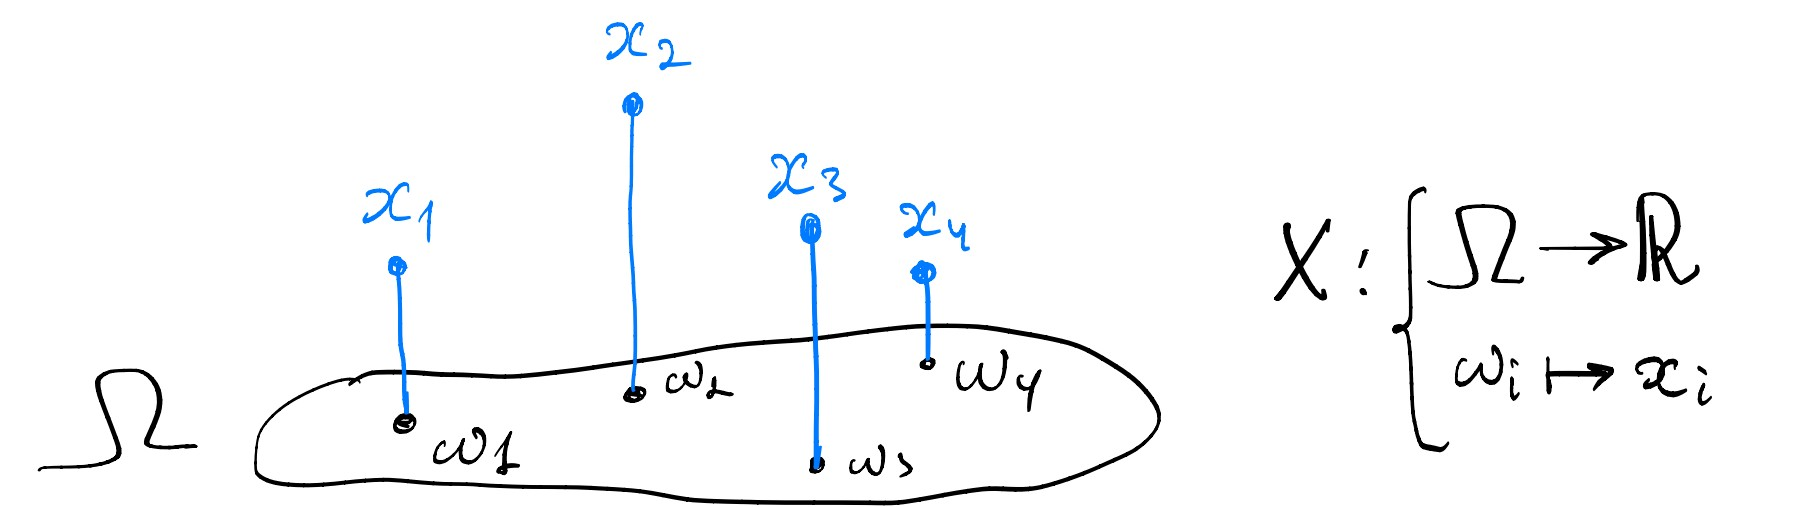
\includegraphics[width=0.8\textwidth]{pictures/random_variable_1.jpg}
    \caption{Задание случайной величины, как функцию от исходов}
\end{figure}

Случайная величина это датчик, который показывает ''температуру'' в разных точках пространства исходов.
Такая склейка исходов суммирует их вероятности. Так,
\[
P(\omega: X_3(\omega) = 1) = P((0,1)) + P((1,0)) = \frac{1}{4} + \frac{1}{4} = \frac{1}{2}.
\]
Если продолжать аналогию с температурой, то точки пространства с одинаковой температурой стали неразличимы, а их суммарная площадь стала больше. И тогда, имея такой датчик, мы можем задавать вопрос: с какой вероятностью муха окажется в точке с температурой 10 градусов?

\threestars
Заметим, что случайная величина задает новое вероятностное пространство.

Обозначим буквой $\mathcal{X}$ множество всех значений случайной величины $X$. То есть
\[
\mathcal{X} = \{x_1, \ldots, x_n\}.
\]
Тогда, замеряя температуру, мы проводим эксперимент с исходами $\mathcal{X}$, а распределение вероятности $P_X$ будет следующим
\[
P_X(x_i) = P(\omega \in \Omega: X(\omega) = x_i)
\]
\note Часто запись $P(\omega \in \Omega: X(\omega) = x_i)$ сокращают до $P(X = x_i)$. Тогда
\[
P_X(x_i) = P(X = x_i).
\]
\begin{figure}[h] % [h] означает "здесь"
    \centering
    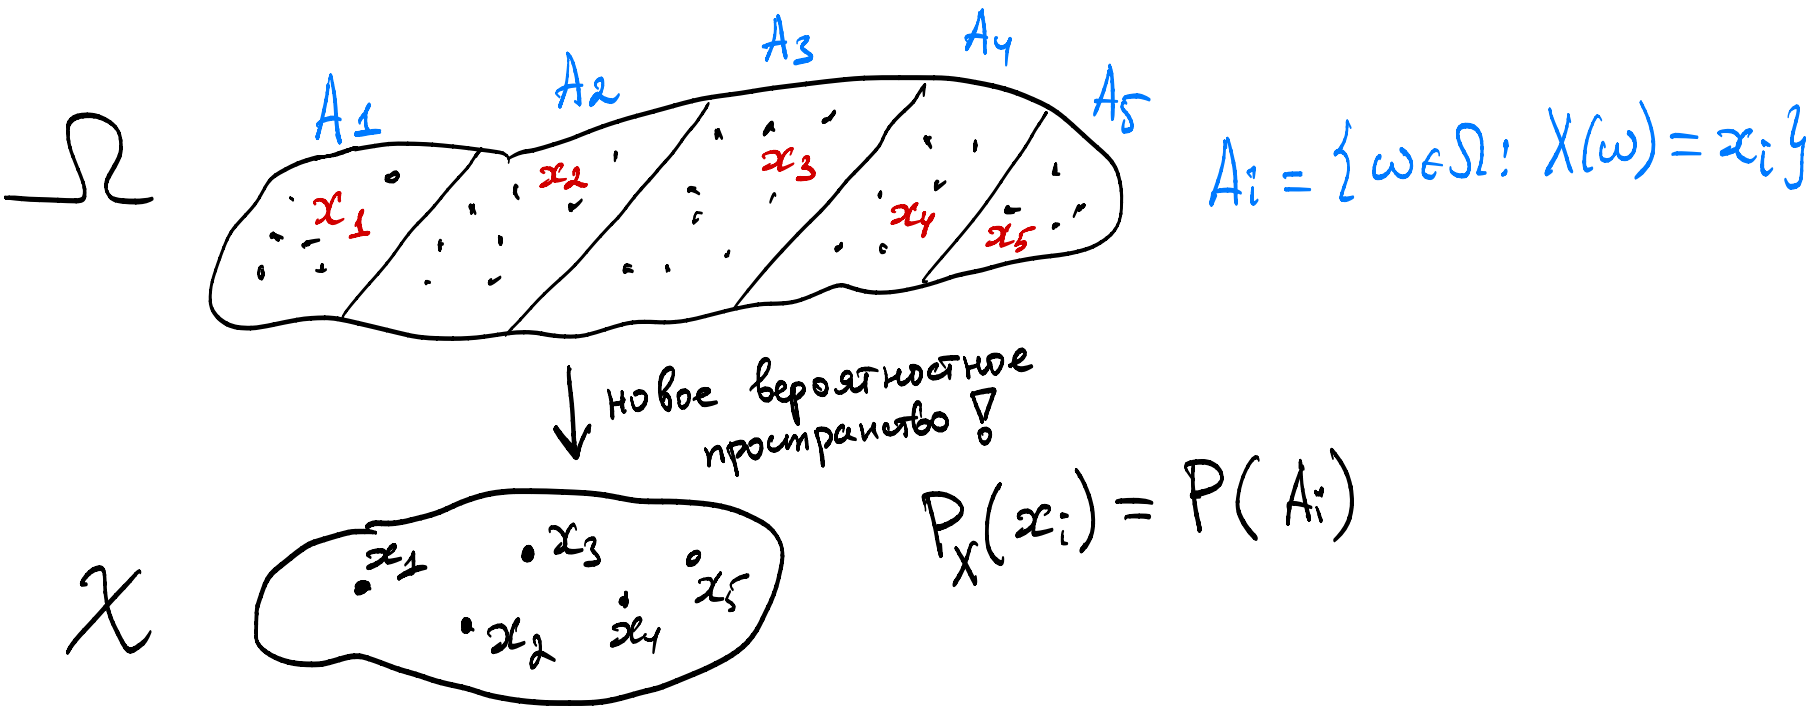
\includegraphics[width=0.8\textwidth]{pictures/random_variable_2.jpg}
\end{figure}
\df Пространство $(\mathcal{X}, 2^\mathcal{X}, P_X)$ называется вероятностным пространством, заданным случайной величиной $X$.

\df Распределение $P_X$ называется распределением случайной величины $X$. 

\notion Если случайная величина $X$ имеет распределение $P$, то пишут \mbox{$X \sim P$}.

\threestars

Распределение случайной величины часто задают в виде таблицы или графика:
\begin{center}
\begin{tabular}{|c|c|c|c|c|c|}
\hline
$x \in \mathcal{X}$ & $x_1$ & $x_2$ & $\cdots$ & $x_{n-1}$ & $x_n$ \\
\hline
$P_X(x)$  & $p_1$ & $p_2$ & $\cdots$ & $p_{n-1}$ & $p_n$ \\
\hline
\end{tabular}
\end{center}

\begin{center}
\begin{tikzpicture}
    \begin{axis}[
        ybar,
        bar width=15pt,
        ymin=0,
        ymax=0.5,
        symbolic x coords={$x_1$, $x_2$, $x_3$, $\cdots$, $x_{n-1}$, $x_n$},
        xtick=data,
        xlabel={$x$},
        ylabel={$P_X(x)$},
        title={$X \sim P_X$},
        grid=both,
        width=12cm,
        height=8cm,
        every axis plot/.append style={fill=blue, opacity=0.7},
    ]
    \addplot+[ybar, fill=blue] coordinates {($x_1$,0.15) ($x_2$,0.25) ($x_3$,0.05) ($\cdots$,0.05) ($x_{n-1}$,0.1) ($x_n$,0.4)};
    \end{axis}
\end{tikzpicture}
\end{center}

\threestars

\NB{На практике нас интересует распределение именно случайной величины, а распределение вероятности на исходном вероятностном пространстве -- нет. Поэтому при исследовании случайных величин даже не обязательно знать $\Omega$, достаточно знать только, что оно есть.}

\begin{exercise}
    Обратимся к примеру с бросанием двух монет и случайным величинам $X_1$, $X_2$, $X_3$. Описать для каждой из них вероятностное пространство $(\mathcal{X}_i, 2^{\mathcal{X}_i}, P_{X_i})$, которое они задают.
\end{exercise}

\threestars

Остановимся на понятии распределения случайной величины.

Распределение -- главная и определяющая характеристика случайной величины, которая говорит о том, с какой вероятностью мы будем наблюдать каждое возможное значение. Попробуем почувствовать это чуть глубже.

Снова представим себя физиком-экспериментатором. Нам надо исследовать некую среду, хоть бы например и помещение, где мы находимся. Тогда мы возьмем любую точку пространства в этом помещении и будем разглядывать ее, пытаясь исследовать ее свойства, а значит и свойства всех остальных точек помещения.

Загвоздка в том, что у точки огромное количество свойств: температура, влажность, скорость ветра, давление воздуха, расстояние до Амстердама, количество проходивших через нее за все время людей и т.д.

Назовем совокупность всех этих свойств состоянием. Это состояние есть у каждой точки, и оно случайно. Напомню, что под случайностью надо понимать субъективную нехватку информации для достоверного знания о чем-либо. А про состояние точки мы что-то знаем, может быть ее положение, а многое не знаем.

Так вот, состояние точки оказывается случайным исходом в нашем уже привычном понимании вероятностного пространства, то бишь вероятностной модели эксперимента:

\begin{align*}
    &\Omega = \{ \text{все возможные состояния} \}\\
    &\mathcal{F} = 2^\Omega\\
    &P - \text{какое-то}.
\end{align*}
Распределение $P$ указывает на то, какие состояния более, а какие менее вероятны.

Но изучать состояния вообще -- неконкретная задача. Непонятно, что именно изучать. Поэтому разумно наблюдать за специфическими свойствами состояния, которые уже можно подвергать анализу.

Естественно выделяются те свойства, которые можно описать количественно, то есть численно. А значит, нужен датчик, реальный или воображаемый (для теоретических исследований), который бы умел вычислять конкретную величину, характеризующую некоторое свойство общего состояние, например температуру.

В этой аналогии с датчиком легко провести все параллели. Итак, само состояние измеряемого объекта это исход $\omega \in \Omega$, значение датчика это $X$, механизм работы датчика это отображение
\[
    X: \Omega \rightarrow \R.
\]
Причем, механизм всегда работает одинаково, но засчет того, что сам исход случаен, то и значение датчика случайно.

Но случайность бывает разная. Рост первого попавшегося прохожего -- случайная величина, но это не значит, что про эту случайность мы ничего не знаем. Например, мы знаем, что скорее всего рост этого человека будет около 160-180 сантиметров.

Поэтому распределение вероятности на обычном вероятностном пространстве или на пространстве, порожденном случайной величиной, это именно описание самой случайности, того, какова эта случайность.

\threestars

\task[(Задача 3.1 из \cite{ZubkovSevostyanovChistyakov1989})] Распределение случайной величины $X$ определяется формулами
\[
P(X=i) = \frac{1}{5}, \quad i = -2,-1,0,1,2.
\]
Найти распределение величин $Y_1 = -X$, $Y_2 = |X|$.

\begin{proof}
    Найдем распределение $Y_1$, записав его в виде таблички:
    \begin{center}
    \begin{tabular}{|c|c|c|c|c|c|}
    \hline
    $k$ & $-2$ & $-1$ & $0$ & $1$ & $2$ \\
    \hline
    $P(Y_1 = k)$ & $1/5$ & $1/5$ & $1/5$ & $1/5$ & $1/5$ \\
    \hline
    \end{tabular}
    \end{center}
    Из интересного заметим, что $Y$ имеет то же самое распределение, что и $X$, но это другая случайная величина, они не равны как функции!

    Аналогично сделаем с величиной $Y_2$:
    \begin{center}
    \begin{tabular}{|c|c|c|c|}
    \hline
    $k$ & $0$ & $1$ & $2$ \\
    \hline
    $P(Y_2 = k)$ & $1/5$ & $2/5$ & $2/5$ \\
    \hline
    \end{tabular}
    \end{center}
\end{proof}

\task[(Задача 3.2 из \cite{ZubkovSevostyanovChistyakov1989})] Распределение случайной величины $X$ определяется формулами
\[
P(X=k) = \frac{C}{k(k+1)}, \quad k = 1,2, \ldots
\]
Найти: а) постоянную $C$; б) $P(X \le 3)$; в) $P(n_1 \le X \le n_2)$.

\begin{proof}
    Чтобы найти $C$, нужно воспользоваться определением $P$:
    \[
    \sum_{k=1}^\infty P(X=k) = 1.
    \]
    То есть должно выполняться равенство
    \[\sum_{k=1}^\infty \frac{C}{k(k+1)} = 1.\]
    Для вычисления этого ряда воспользуемся тем, что
    \[
    \frac{1}{k(k+1)} = \frac{1}{k} - \frac{1}{k+1}.
    \]
    Тогда
    \[
    \sum_{k=1}^\infty \frac{1}{k(k+1)} = \braces{1 - \frac{1}{2}} + \braces{\frac{1}{2} - \frac{1}{3}} + \braces{\frac{1}{3} - \frac{1}{4}} + \cdots = 1.
    \]
    А значит
    \[\sum_{k=1}^\infty \frac{C}{k(k+1)} = C = 1,\]
    то есть $C=1$.

    Теперь вычислим $P(X\le 3)$:
    \begin{align*}
        P(X \le 3) &= P(X=1) + P(X=2) + P(X=3) =\\
        &=\frac{1}{2} + \frac{1}{6} + \frac{1}{12} = \frac{3}{4}.
    \end{align*}

    И осталось посчитать $P(n_1 \le X \le n_2)$:
    \begin{align*}
        P(n_1 \le X \le n_2) &= \sum_{k=n_1}^{n_2} P(X=k) = \sum_{k=n_1}^{n_2} \braces{\frac{1}{k} - \frac{1}{k+1}} =\\
        & = \braces{\frac{1}{n_1} - \frac{1}{n_1+1}} + \braces{\frac{1}{n_1+1} - \frac{1}{n_1+2}} + \cdots + \braces{\frac{1}{n_2} - \frac{1}{n_2+1}} =\\
        & = \frac{1}{n_1} - \frac{1}{n_2+1} = \frac{n_2-n_1+1}{n_1(n_2+1)}.
    \end{align*}
\end{proof}

\ex $X$ -- случайная величиная, задающая число бросков монеты до последнего выпадения орла среди 10 бросков монеты с вероятностью орла $p$ (если орлов не было, то величина равна 0). Построить $\mathcal{X}$, найти распределение $X$, найти $P(X<3)$.

\begin{proof}
    $X$ может принимать значения
    \[
    \mathcal{X} = \{0,1, \ldots, 10\}.
    \]
    Случайная величина задана на вероятностном пространстве. Определим для удобства в дальнейшем множество исходов:
    \[
    \Omega = \{ (a_1, \ldots, a_{10}): a_i \in \{O,P\} \}.
    \]
    Теперь найдем распределение $X$. Для этого нужно вычислить вероятности $P(X = i)$, где $i \in \mathcal{X}$. Итак,
    \[
    P(X = 0) = (1-p)^{10},
    \]
    так как это означает, что выпали только решки.

    Далее, событие $X = 1$ означает, что первым выпал орел и дальше были только решки, т.е.
    \[
    P(X = 1) = p(1-p)^9.
    \]
    Событие $X=2$ означает, что вторым выпал орел, дальше только решки. А на первом месте могло быть что угодно. Распишем это по формуле полной вероятности
    \begin{align*}
        P(X=2) &= P(X=2 \mid a_1 = O)P(a_1=O) + P(X=2 \mid a_1 = P)P(a_1=P) = \\
        & = p(1-p)^8 \cdot p + p(1-p)^8 \cdot (1-p) = p(1-p)^8. 
    \end{align*}

    Аналогично, для $X=3$ можно разбить на случаи по всем возможным исходам первых двух бросков. Получим
    \[
    P(X=3) = p(1-p)^7.
    \]
    И так далее
    \[
    P(X=i) = p(1-p)^{10-i}, \quad i = 1,\ldots 10.
    \]
    Таким образом, распределение $X$ найдено.
    \begin{center}
        \begin{tikzpicture}
            \begin{axis}[
                ybar, % Гистограмма
                bar width=12pt, % Ширина столбцов
                ymin=0, % Минимальное значение оси Y
                ymax=0.35, % Максимальное значение оси Y
                xmin=-1, % Минимальное значение оси X
                xmax=11, % Максимальное значение оси X
                xtick=data, % Отображение отметок по X
                xlabel={$k$}, % Подпись к оси X
                ylabel={$P(X = k)$}, % Подпись к оси Y
                title={Распределение $X$ при $p=0.3$}, % Заголовок графика
                grid=both, % Включение сетки
                width=12cm, % Ширина графика
                height=8cm, % Высота графика
                every axis plot/.append style={fill=blue, opacity=0.7}, % Цвет и прозрачность
            ]
            \addplot+[ybar, fill=blue] plot coordinates {
                % автоматический расчёт значений для k=0..25
                % PGFPlots сам будет вычислять формулу
                % Формула: exp(-λ) * λ^k / k!
                % здесь λ = 6
                % цикл по k
                (0, {(1-0.3)^(10)})
                (1, {0.3*(1-0.3)^9})
                (2, {0.3*(1-0.3)^8})
                (3, {0.3*(1-0.3)^7})
                (4, {0.3*(1-0.3)^6})
                (5, {0.3*(1-0.3)^5})
                (6, {0.3*(1-0.3)^4})
                (7, {0.3*(1-0.3)^3})
                (8, {0.3*(1-0.3)^2})
                (9, {0.3*(1-0.3)^1})
                (10, {0.3*(1-0.3)^0})
            };
            \end{axis}
        \end{tikzpicture}
    \end{center}

    Вероятность события $X<3$, т.е. того, что последний орел выпал не позже второго броска, считается просто:
    \begin{align*}
        P(X<3) &= P(X=0) + P(X=1) + P(X=2) = \\
        & = (1-p)^{10} + p(1-p)^9 + p(1-p)^8 = \\
        & = (1-p)^8 ((1-p)^2 + p(1-p) + p) = \\
        & = (1-p)^8.
    \end{align*}
\end{proof}


\subsection*{Базовые распределения}\addcontentsline{toc}{subsection}{Базовые распределения}
Распределение случайной величины описывает математическую модель эксперимента, как и в случае с вероятностным пространством. Но, как уже было сказано, случайная величина указывает не на любые исходы, а на численные показатели исхода.

В этом разделе мы рассмотрим базовые распределения, которые чаще всего встречаются в моделировании.

\subsubsection*{Равномерное распределение, $X \sim U\{1, \ldots, N\}$}\addcontentsline{toc}{subsubsection}{Равномерное распределение, $X \sim U\{0, \ldots, N\}$}

Равномерное распределение соответствует эксперименту, где все значения случайной величины равновероятны. Тогда все возможные значения это
\[
\mathcal{X} = \{1, \ldots, N\},
\]
с распределением
\[
P_X(k) = \frac{1}{N}, \quad 1\le k \le N.
\]
\begin{center}
\begin{tikzpicture}
    \begin{axis}[
        ybar,
        bar width=15pt,
        ymin=0,
        ymax=0.2,
        xmin=0,
        xmax=9,
        xtick={1,...,8},
        xlabel={$k$},
        ylabel={$P(X = k)$},
        title={$X \sim U\{1,\dots,N\}, \quad N = 8$},
        grid=both,
        width=12cm,
        height=8cm,
        every axis plot/.append style={fill=blue, opacity=0.7},
    ]
    \addplot+[ybar, fill=blue] plot coordinates {
        (1, {1/8})
        (2, {1/8})
        (3, {1/8})
        (4, {1/8})
        (5, {1/8})
        (6, {1/8})
        (7, {1/8})
        (8, {1/8})
    };
    \end{axis}
\end{tikzpicture}
\end{center}

Например, такая величина описывает количество очков, которое выпадет на шестигранном кубике, или номер шара, который вынут из урны.

\subsubsection*{Распределение Бернулли, $X \sim Bern(p)$}\addcontentsline{toc}{subsubsection}{Распределение Бернулли, $X \sim Bern(p)$}
Это распределение моделирует подбрасывание несимметричной монетки, или, более абстрактно, любого эксперимента, где есть только два исхода: успех и неудача, причем вероятность успеха равна $p$.

Таким образом, множество значений случайной величины есть
\[
\mathcal{X} = \{0, 1\},
\]
а распределение таково
\begin{align*}
    &P_X(1) = p\\
    &P_X(0) = 1-p. 
\end{align*}

Распределение названо в честь Якоба Бернулли, одного из основоположников теории вероятностей. Он изучал в основном именно такие эксперименты с двумя исходами и доказал для этого случая вариант закона больших чисел.

\begin{center}
    \begin{tikzpicture}
        \begin{axis}[
            ybar, % Гистограмма
            bar width=28pt, % Ширина столбцов
            ymin=0, % Минимальное значение оси Y
            ymax=1, % Максимальное значение оси Y
            xmin=-1, % Минимальное значение оси X
            xmax=2, % Максимальное значение оси X
            xtick=data, % Отображение отметок по X
            xlabel={$k$}, % Подпись к оси X
            ylabel={$P(X = k)$}, % Подпись к оси Y
            title={$X \sim Bern(p)$, $p=0.6$}, % Заголовок графика
            grid=both, % Включение сетки
            width=12cm, % Ширина графика
            height=8cm, % Высота графика
            every axis plot/.append style={fill=blue, opacity=0.7}, % Цвет и прозрачность
        ]
        \addplot[
            ybar,
            fill=blue,
        ] table[row sep=\\] {
            k   P \\
            0   0.4 \\
            1   0.6 \\
        };
        \end{axis}
    \end{tikzpicture}
\end{center}

\subsubsection*{Биномиальное распределение, $X \sim Binom(n, p)$}\addcontentsline{toc}{subsubsection}{Биномиальное распределение, $X \sim Binom(n, p)$}
Биномиальное распределение моделирует количество успехов в $n$ независимых испытаниях. Таким образом, множество значений случайной величины $X$ есть
\[
\mathcal{X} = \{0, 1, \ldots, n\},
\]
а распределение $X$ будет следующим:
\[
P_X(k) = C_n^k p^k (1-p)^{n-k}.
\]
\begin{center}
    \begin{tikzpicture}
        \begin{axis}[
            ybar, % Гистограмма
            bar width=8pt, % Ширина столбцов
            ymin=0, % Минимальное значение оси Y
            ymax=0.2, % Максимальное значение оси Y
            xmin=0, % Минимальное значение оси X
            xmax=20, % Максимальное значение оси X
            xtick=data, % Отображение отметок по X
            xlabel={$k$}, % Подпись к оси X
            ylabel={$P(X = k)$}, % Подпись к оси Y
            title={$X \sim Binom(n, p), \quad n=20, \ p=0.55$}, % Заголовок графика
            grid=both, % Включение сетки
            width=12cm, % Ширина графика
            height=8cm, % Высота графика
            every axis plot/.append style={fill=orange, opacity=0.7}, % Цвет и прозрачность
        ]
        \addplot[
            ybar,
            fill=blue,
        ] table[row sep=\\] {
            k   P \\
            0   0.0000 \\
            1   0.0000 \\
            2   0.0001 \\
            3   0.0005 \\
            4   0.0021 \\
            5   0.0069 \\
            6   0.0185 \\
            7   0.0414 \\
            8   0.0804 \\
            9   0.1306 \\
            10  0.1767 \\
            11  0.1964 \\
            12  0.1797 \\
            13  0.1321 \\
            14  0.0776 \\
            15  0.0370 \\
            16  0.0135 \\
            17  0.0039 \\
            18  0.0008 \\
            19  0.0001 \\
            20  0.0000 \\
        };
        \end{axis}
    \end{tikzpicture}
\end{center}

\subsubsection*{Геометрическое распределение, $X \sim Geom(p)$}\addcontentsline{toc}{subsubsection}{Геометрическое распределение, $X \sim Geom(p)$}
Случайная величина $X \sim Geom(p)$ моделирует число неудач до первого успеха, когда вероятность успеха равна $p$. Таким образом, множество значений $X$ есть
\[
\mathcal{X} = \{0, 1, 2, \ldots\} = \mathbb{N} \cup \{0\},
\]
а распределение будет иметь вид
\[
P_X(k) = p(1-p)^k.
\]
\begin{center}
    \begin{tikzpicture}
        \begin{axis}[
            ybar, % Гистограмма
            bar width=8pt, % Ширина столбцов
            ymin=0, % Минимальное значение оси Y
            ymax=0.4, % Максимальное значение оси Y
            xmin=-1, % Минимальное значение оси X
            xmax=15, % Максимальное значение оси X
            xtick=data, % Отображение отметок по X
            xlabel={$k$}, % Подпись к оси X
            ylabel={$P(X = k)$}, % Подпись к оси Y
            title={$X \sim Geom(p)$, $p=0.3$}, % Заголовок графика
            grid=both, % Включение сетки
            width=12cm, % Ширина графика
            height=8cm, % Высота графика
            every axis plot/.append style={fill=blue, opacity=0.7}, % Цвет и прозрачность
        ]
        \addplot[
            ybar,
            fill=blue,
        ] table[row sep=\\] {
            k   P \\
            0   0.3 \\
            1   0.21 \\
            2   0.147 \\
            3   0.1029 \\
            4   0.07203 \\
            5   0.050421 \\
            6   0.0352947 \\
            7   0.0247063 \\
            8   0.0172944 \\
            9   0.0121061 \\
            10  0.0084743 \\
            11  0.005932 \\
            12  0.0041524 \\
            13  0.0029067 \\
            14  0.0020347 \\
        };
        \end{axis}
    \end{tikzpicture}
\end{center}
Геометрическим это распределение называется потому, что сумма
\[
\sum_{k=0}^\infty P_X(k) = p\sum_{k=0}^\infty (1-p)^k = \frac{p}{1-(1-p)} = 1
\]
является геометрической прогрессией.

\subsubsection*{Распределение Пуассона, $X \sim Poisson(\lambda)$}\addcontentsline{toc}{subsubsection}{Распределение Пуассона, $X \sim Poisson(\lambda)$}
Пуассоновское распределение моделирует количество событий, произошедших за некоторое время, причем о событии известно среднее количество $\la$ его появлений за этот промежуток времени.

Итак, множество значений величины $X \sim Poisson(\la)$ будет
\[
\mathcal{X} = \{0,1,2, \ldots\},
\]
а распределение задается следующим образом
\[
P_X(k) = \frac{\la^k}{k!} e^{-\la}, \quad \la > 0.
\]

\begin{center}
\begin{tikzpicture}
    \begin{axis}[
        ybar,
        bar width=8pt,
        ymin=0,
        ymax=0.18,
        xmin=-1,
        xmax=26,
        xtick={0,...,25},
        xlabel={$k$},
        ylabel={$P(X = k)$},
        title={$X \sim \text{Poisson}(\lambda=6)$},
        grid=both,
        width=14cm,
        height=8cm,
        every axis plot/.append style={fill=blue, opacity=0.7},
    ]
    \addplot+[ybar, fill=blue] plot coordinates {
        % автоматический расчёт значений для k=0..25
        % PGFPlots сам будет вычислять формулу
        % Формула: exp(-λ) * λ^k / k!
        % здесь λ = 6
        % цикл по k
        (0, {exp(-6)*6^0/factorial(0)})
        (1, {exp(-6)*6^1/factorial(1)})
        (2, {exp(-6)*6^2/factorial(2)})
        (3, {exp(-6)*6^3/factorial(3)})
        (4, {exp(-6)*6^4/factorial(4)})
        (5, {exp(-6)*6^5/factorial(5)})
        (6, {exp(-6)*6^6/factorial(6)})
        (7, {exp(-6)*6^7/factorial(7)})
        (8, {exp(-6)*6^8/factorial(8)})
        (9, {exp(-6)*6^9/factorial(9)})
        (10, {exp(-6)*6^10/factorial(10)})
        (11, {exp(-6)*6^11/factorial(11)})
        (12, {exp(-6)*6^12/factorial(12)})
        (13, {exp(-6)*6^13/factorial(13)})
        (14, {exp(-6)*6^14/factorial(14)})
        (15, {exp(-6)*6^15/factorial(15)})
        (16, {exp(-6)*6^16/factorial(16)})
        (17, {exp(-6)*6^17/factorial(17)})
        (18, {exp(-6)*6^18/factorial(18)})
        (19, {exp(-6)*6^19/factorial(19)})
        (20, {exp(-6)*6^20/factorial(20)})
        (21, {exp(-6)*6^21/factorial(21)})
        (22, {exp(-6)*6^22/factorial(22)})
        (23, {exp(-6)*6^23/factorial(23)})
        (24, {exp(-6)*6^24/factorial(24)})
        (25, {exp(-6)*6^25/factorial(25)})
    };
    \end{axis}
\end{tikzpicture}
\end{center}

Примеров, которые описывались бы пуассоновской случайной величиной, много. Нужно, чтобы события были маловероятными, но при этом их было достаточно много. Например, число автомобильных аварий в Москве за день, число забиваемых голов и т.д.

Полезный источник: \href{https://education.yandex.ru/handbook/ml/article/veroyatnostnye-raspredeleniya}{учебник Яндекса по ML}.

\subsection*{Совместные распределения}\addcontentsline{toc}{subsection}{Совместные распределения}
Если на одном вероятностном пространстве $(\Omega, \mathcal{F}, P)$ задано несколько случайных величин $X_1, \ldots, X_n$, то говорят, что на этом вероятностном пространстве задан случайный вектор $(X_1, \ldots, X_n)$.

Такой случайный вектор задает новое вероятностное пространство
\[
\mathcal{X} = \mathcal{X}_1 \times \cdots \times \mathcal{X}_n, \quad \mathcal{F}_X = 2^\mathcal{X}
\]
с вероятностной мерой $P_X$, заданной формулой
\[
P_X((x_{1, i_1}, \ldots, x_{n,i_n})) = P(X_1 = x_{1,i_1}, \ldots, X_n = x_{n,i_n}).
\]
Эта мера называется совместным распределением случайных величин $X_1, \ldots X_n$.

\task[(Задача 3.16 из \cite{ZubkovSevostyanovChistyakov1989})] Совместное распределение $p_{ij} = P(X_1 = i, X_2 = j)$ случайных величин $X_1$, $X_2$ задано таблицей:
\begin{center}
\begin{tabular}{|c|c|c|c|}
\hline
\diagbox{$X_1$}{$X_2$} & -1 & 0 & 1 \\ \hline
-1 & 1/8 & 1/12 & 7/24 \\ \hline
1 & 5/24 & 1/6 & 1/8 \\ \hline
\end{tabular}
\end{center}
Найти a) одномерные распределения $p_i = P(X_1=i)$ и $p_j = P(X_2=j)$; б) совместное распределение $q_{ij} = P(Y_1 = i, Y_2=j)$ случайных величин $Y_1 = X_1+X_2$, $Y_2 = X_1 X_2$, в) одномерные распределения $q_i = P(Y_1 = i)$, $q_j=P(Y_2=j)$.

\begin{proof}
    Пункт а). Найдем $P(X_1 = -1)$. Для этого воспользуемся разбиением этого события (почти формула полной вероятности):
    \begin{align*}
        P(X_1 = -1) &= P(X_1=-1, X_2 = -1) + P(X_1=-1, X_2 = 0) + P(X_1 = -1, X_2 = 1) =\\
        &= \frac{1}{8} + \frac{1}{12} + \frac{7}{24} = \frac{1}{2}.
    \end{align*}
    Отсюда становится понятно, что маргинальные распределения легко найти из таблички совместного распределения путем простого сложения вероятностей по строчкам или столбцам.

    Теперь легко получаем:
    \begin{align*}
        &P(X_1 = 1) = \frac{5}{24} + \frac{1}{6} + \frac{7}{24} = \frac{1}{2}\\
        &P(X_2 = -1) = \frac{1}{8} + \frac{5}{24} = \frac{1}{3}\\
        &P(X_2 = 0) = \frac{1}{12} + \frac{1}{6} = \frac{1}{4}\\
        &P(X_2 = 1) = \frac{7}{24} + \frac{1}{8} = \frac{5}{12}.
    \end{align*}

    Пункт б). Теперь найдем совместное распределение величин $Y_1$ и $Y_2$. Для этого по сути нужно заполнить табличку
    \begin{center}
    \begin{tabular}{|c|c|c|c|}
    \hline
    \diagbox{$Y_1$}{$Y_2$} & -1 & 0 & 1 \\ \hline
    -2 & & & \\ \hline
    -1 & & & \\ \hline
    0 & & & \\ \hline
    1 & & & \\ \hline
    2 & & & \\ \hline
    \end{tabular}
    \end{center}
    Начнем.
    \begin{align*}
    P(Y_1 = -2, Y_2 = -1) &= P(X_1+X_2 = -2, X_1X_2 = -1) =\\
    &= P(X_1 = -1, X_2 = -1, X_1X_2 = -1) = 0.
    \end{align*}
    Далее, уже очевидно, что
    \begin{align*}
        &P(Y_1 = -2, Y_2 = 0) = 0,\\
        &P(Y_1 = -2, Y_2 = 1) = P(X_1 = -1, X_2 = -1) = \frac{1}{8}.
    \end{align*}
    Таким образом, первую строчку заполнили.

    Далее, так как $Y_1 = -1 \Leftrightarrow X_1 = -1, X_2 = 0$, то получаем вторую строчку таблицы
    \begin{align*}
        &P(Y_1 = -1, Y_2 = -1) = 0,\\
        &P(Y_1 = -1, Y_2 = 0) = P(X_1 = -1, X_2 = 0) = \frac{1}{12},\\
        &P(Y_1 = -1, Y_2 = 1) = 0.
    \end{align*}
    Для третьей строки таблицы заметим, что $Y_1 = 0 \Leftrightarrow X_1 = -1, X_2 = 1$ или $X_1 = 1, X_2 = -1$. Тогда
    \begin{align*}
        &P(Y_1 = 0, Y_2 = -1) = P(X_1 = -1, X_2 = 1) + P(X_1 = 1, X_2 = -1) = \frac{7}{24} + \frac{5}{24} = \frac{1}{2},\\
        &P(Y_1 = 0, Y_2 = 0) = 0,\\
        &P(Y_1 = 0, Y_2 = 1) = 0.
    \end{align*}
    Для четвертой строчки: $Y_1 = 1 \Leftrightarrow X_1 = 1, X_2 = 0$, поэтому
    \begin{align*}
        &P(Y_1 = 1, Y_2 = -1) = 0,\\
        &P(Y_1 = 1, Y_2 = 0) = P(X_1 = 1, X_2 = 0) = \frac{1}{6},\\
        &P(Y_1 = 1, Y_2 = 1) = 0.
    \end{align*}
    И наконец для пятой строчки $Y_1 = 2 \Leftrightarrow X_1 = 1, X_2 = 1$, значит,
    \begin{align*}
        &P(Y_1 = 2, Y_2 = -1) = 0,\\
        &P(Y_1 = 2, Y_2 = 0) = 0,\\
        &P(Y_1 = 2, Y_2 = 1) = P(X_1 = 1, X_2 = 1) = \frac{1}{8}.
    \end{align*}
    Итого, получаем совместное распределение $Y_1$ и $Y_2$:
    \begin{center}
    \begin{tabular}{|c|c|c|c|}
    \hline
    \diagbox{$Y_1$}{$Y_2$} & -1 & 0 & 1 \\ \hline
    -2 & 0 & 0 & 1/8 \\ \hline
    -1 & 0 & 1/12 & 0 \\ \hline
    0 & 1/2 & 0 & 0 \\ \hline
    1 & 0 & 1/6 & 0 \\ \hline
    2 & 0 & 0 & 1/8 \\ \hline
    \end{tabular}
    \end{center}

    Пункт в) Маргинальные распределения тогда находятся легко:
    \begin{center}
    \begin{tabular}{|c|c|c|c|c|c|}
    \hline
    $i$ & -2 & -1 & 0 & 1 & 2 \\ \hline
    $P(Y_1 = i)$ & 1/8 & 1/12 & 1/2 & 1/6 & 1/8 \\ \hline
    \end{tabular}
    \end{center}
    
    \begin{center}
    \begin{tabular}{|c|c|c|c|}
    \hline
    $j$ & -1 & 0 & 1 \\ \hline
    $P(Y_2 = j)$ & 1/2 & 1/4 & 1/4 \\ \hline
    \end{tabular}
    \end{center}

\end{proof}

\task[] Привести пример, когда нельзя однозначно восстановить совместное распределение по маргинальным.
\begin{proof}
    Пусть $X_1$, $X_2$ -- случайные величины с распределениями $Bern(1/2)$:
    \begin{align*}
        &P(X_1 = 0) = P(X_1 = 1) = 1/2,\\
        &P(X_2 = 0) = P(X_2 = 1) = 1/2.
    \end{align*}
    Тогда нужно подобрать числа в таблицу совместного распределения, чтобы все суммы сходились. Это легко сделать (попробуйте сами):
    \begin{center}
    \begin{tabular}{|c|c|c|}
    \hline
    \diagbox{$X_1$}{$X_2$} & 0 & 1 \\ \hline
    0 & 1/6 & 1/3 \\ \hline
    1 & 1/3 & 1/6 \\ \hline
    \end{tabular}
    \hspace{1cm}
    \begin{tabular}{|c|c|c|}
    \hline
    \diagbox{$X_1$}{$X_2$} & 0 & 1 \\ \hline
    0 & 1/2 & 0 \\ \hline
    1 & 0 & 1/2 \\ \hline
    \end{tabular}
    \end{center}
\end{proof}

\task[(Задача 3.49 из \cite{ZubkovSevostyanovChistyakov1989})] В схеме Бернулли с вероятностью успеха $p$ обозначим $\nu_k$ ($k=1, 2, \ldots$) номер испытания, при котором происходит $k$-й успех, и положим 
\[\tau_1 = \nu_1,\quad \tau_k = \nu_k - \nu_{k-1}\quad(k=2, 3,\ldots).\]
Найти совместное распределение величин $\tau_1, \tau_k$. Являются ли эти величины независимыми?

\begin{proof}
    Введем случайные величины $X_i \sim Bern(p)$ -- результат $i$ испытания. Тогда
    \begin{align*}
        P(\tau_1 = l_1, \tau_k = l_2) = P(&X_1 = 0, \ldots, X_{l_1-1} = 0, X_{l_1} = 1, \\
        &X_{\nu_{k-1}} = 0, \ldots, X_{\nu_{k-1} + l_2-1} = 0, X_{\nu_k} = 1) =\\
        &= (1-p)^{l_1-1} p \cdots (1-p)^{l_2-1}p = (1-p)^{l_1 + l_2 -2} p^2.
    \end{align*}
    При этом
    \[
    P(\tau_1 = l_1, \tau_k = l_2) = P(\tau_1 = l_1) P(\tau_k = l_2),
    \]
    значит, величины $\tau_1$ и $\tau_k$ независимы.
\end{proof}

\task[(Задача 3.51 из \cite{ZubkovSevostyanovChistyakov1989})] Игральную кость бросают до того момента, когда впервые выпадает меньше пяти очков. Обозначим через $\theta$ число очков, выпавших при последнем бросании игральной кости, и через $\nu$ -- число бросаний кости. Найти совместное распределение $\theta$ и $\nu$. Являются ли случайные величины $\theta$ и $\nu$ зависимыми?

\begin{proof}
    Определимся с тем, какие значения принимают случайные величины $\theta$ и $\nu$. Ясно, что
    \[
    \theta \in \{1,2,3,4\}, \quad \nu \in \{1,2,3\ldots\}.
    \]
    Нам нужно найти вероятности $P(\theta = i, \nu = j)$. Событие $\{\theta = i, \nu = j\}$ означает, что $j-1$ раз выпадали числа $\ge 5$, а на $j$-ый раз выпало $i$. Так как последовательные бросания кости считаются независимыми, то получаем, что вероятность этого события равна
    \[
    P(\theta = i, \nu = j) = \braces{\frac{2}{6}}^{j-1} \cdot \frac{1}{6} = \frac{1}{6} \braces{\frac{1}{3}}^{j-1}.
    \]
    В задачнике предлагается выразить то же событие в терминах новой случайной величины $\xi_i$ -- результат $i$-го броска кубика. Тогда получим
    \begin{align*}
        P(\theta = i, \nu = j) &= P(\xi_1, \ldots, \xi_{j-1} \le 4,\ \xi_j = i) =\\
        &= \braces{\frac{2}{6}}^{j-1} \cdot \frac{1}{6} = \frac{1}{6} \braces{\frac{1}{3}}^{j-1}.
    \end{align*}
    Найдем маргинальные распределения.
    \begin{align*}
        P(\theta = i) = \sum_{j=1}^\infty \frac{1}{6} \braces{\frac{1}{3}}^{j-1} = \frac{1}{6} \cdot \frac{1}{1 - \frac{1}{3}} = \frac{1}{4}.
    \end{align*}
    И для $\nu$:
    \[
    P(\nu = j) = \sum_{i=1}^4 P(\theta = i, \nu = j) = 4 \cdot \frac{1}{6} \braces{\frac{1}{3}}^{j-1} = \frac{2}{3} \braces{\frac{1}{3}}^{j-1}.
    \]
    Отсюда мы видим, что выполняется равенство
    \[
    P(\theta = i, \nu = j) = P(\theta = i)P(\nu = j),
    \]
    значит, величины $\theta$ и $\nu$ независимы.
\end{proof}

\subsection*{Математическое ожидание и дисперсия}\addcontentsline{toc}{subsection}{Математическое ожидание и дисперсия}

Представим, случайная величина $X$ с распределением
\begin{center}
\begin{tabular}{|c|c|c|c|c|c|}
\hline
$x$ & $x_1$ & $x_2$ & $\cdots$ & $x_{n-1}$ & $x_n$ \\ \hline
$P(X = x)$ & $p_1$ & $p_2$ & $\cdots$ & $p_{n-1}$ & $p_n$ \\ \hline
\end{tabular}
\end{center}
замеряется $N$ раз. Будем считать, что у нас $N$ случайных величин $X_1, \ldots, X_N$. Каково будет среднее арифметическое всех результатов? 

Разумно предположить следующую логику. Величины $p_i$ интуитивно должны означать долю испытаний, когда $X$ приняло значение $x_i$. То есть за $N$ повторений мы будем ожидать $N\cdot p_i$ раз, когда выпадет $x_i$. Тогда среднее арифметическое будет таким
\[
\frac{X_1 + X_2 + \cdots + X_N}{N} \approx \frac{x_1 \cdot Np_1 + x_2 \cdot Np_2 + \cdots + x_n \cdot Np_n}{N} = x_1 p_1 + x_2 p_2 + \cdots x_n p_n.
\]

\df Число
\[
EX = x_1 p_1 + x_2 p_2 + \cdots x_n p_n
\]
называется математическим ожиданием случайной величины $X$ (expectation).

\df Число
\[
var X = E(X-EX)^2
\]
называется дисперсией случайной величины $X$ (variance).

\subsection*{Закон больших чисел}\addcontentsline{toc}{subsection}{Закон больших чисел}

\subsection*{Центральная предельная теорема}\addcontentsline{toc}{subsection}{Центральная предельная теорема}

\subsection*{Задачи}\addcontentsline{toc}{subsection}{Задачи}
\task[(Рулетка)] В комнате $n$ человек, у каждого револьвер, по звонку каждый стреляет в случайного человека (кроме себя). Пусть  $X_n$ --- число выживших. Найти $EX_n$.

\begin{proof}
    Введем $Y_i$:
    \[
    Y_i =
    \begin{cases} 
        1, & \text{если i-ый выжил}, \\
        0, & \text{если i-ый не выжил}
    \end{cases}
    \]
    Тогда $X_n = \sum_{k=1}^n Y_k$ и $EX_n = \sum_{k=1}^n EY_n$.

    $$EY_k = P(\text{k-ый выжил})$$

    Чтобы посчитать вероятность, нужно задать вероятностное пространство. Зададим
    $$\Omega = \{(x_1,\ldots, x_n) : x_i \neq i\}$$

    Тогда 
    \begin{align*}
        EY_k &= P(\text{k-ый выжил}) = \frac{(n-2)\cdots(n-2)(n-1)(n-2)\cdots (n-2)}{(n-1)^n} = \\
        &= \frac{(n-2)^{n-1}(n-1)}{(n-1)^n} = \braces{\frac{n-2}{n-1}}^{n-1}
    \end{align*}

    Значит,
    $$EX_n = n\cdot \braces{\frac{n-2}{n-1}}^{n-1}$$

    Отсюда можно заметить, что доля выживших
    $$\frac{EX_n}{n} = \braces{\frac{n-2}{n-1}}^{n-1} = \braces{1-\frac{1}{n-1}}^{n-1} \rightarrow \frac{1}{e}.$$
\end{proof}

\section*{Сюжеты}\addcontentsline{toc}{section}{Сюжеты}
\subsection*{Счастливые билеты}\addcontentsline{toc}{subsection}{Счастливые билеты}

Счастливым билетом считается билет, у которого сумма первых трех цифр совпадает с суммой последних трех цифр. Номера билетов бывают от 000000 до 999999. Задача состоит в том, чтобы найти вероятность того, что человеку, севшему в трамвай, попадется счастливый билет.

При решении этой задачи выяснилось, что ей посвящено несколько статей в журнале ''Квант'' и еще несколько интересных статей с другими подходами к решению.

Возникла идея собрать все это вместе в единый сюжет, объединяющий в себе сразу несколько любопытнейших тем. Здесь будут и признаки делимости, и реккурентные соотношения, и производящие фукнции, и даже интегралы. А в более сложных обобщениях этой задачи применяется даже Центральная предельная теорема.

При этом допускается решение и более менее в лоб. Впрочем, кто-то с этим утверждением поспорит. Об этом решении мы тоже поговорим, но не сразу. Будем идти по нарастающей в смысле сложности техники.

Итак, начнем мы с того, что обратимся к статье \cite{TalkInTram}. 

Понятно, что самое простое, что можно придумать, это перебор: просто перебрать весь миллион вариантов, проверить каждый, подсчитать и дать ответ. Имея компьютер, это сделать совсем просто. Но задача возникла раньше, когда трамваи и автобусы уже были, а компьютеров в каждом доме не было.

Как же можно себе упростить жизнь?

\textbf{Соображения делимости}

\textbf{Утв.} Если суммы цифр двух чисел $a$ и $b$ совпадают, то равны их остатки от деления на 9, т.е. $a \equiv b \pmod{9}$.
\begin{smallproof}
    Рассмотрим трехзначные числа для краткости записи.
    \begin{align*}
        &a = 100k_1 + 10l_1 + m_1\\
        &b = 100k_2 + 10l_2 + m_2
    \end{align*}

    Но тогда сразу получаем, что
    \begin{align*}
        &a = k_1 + l_1 + m_1 \pmod 9\\
        &b = k_2 + l_2 + m_2 \pmod 9
    \end{align*}

    То есть при взятии остатка от деления на 9 числа дают просто сумму цифр. Значит, если равна сумма цифр, то равны и остатки.
\end{smallproof}

Тогда посчитаем, сколько билетиков будут удовлетворять свойству равенства первого и второго трехзначных чисел по модулю 9. Такие билетики назовем красивыми.

Сколько трехзначных чисел дают остаток 0 при делении на 9, т.е. попросту делятся на 9? Таких ненулевых чисел $999/9 = 111$. И еще 000. Тогда билетиков, у которых первая половина делится на 9 и вторая половина делится на 9, будет $112^2 = 12544$.

Трехзначных чисел, дающих остаток 1, будет опять 111 (все те же, что давали остаток на ноль, только с прибавкой единицы, и без $999+1 = 1000$). Значит, билетиков, у которых обе части дают остаток 1 при делении на 9, будет $111^2 = 12321$. И аналогично со всеми остатками до 8.

Таким образом, красивых билетиков будет
\[
12321 \cdot 8 + 12544 = 111112.
\]

\threestars

Итак, мы получили, что счастливых билетиков не больше, чем 111112. Но можно эту оценку улучшить.

\textbf{Утв.} Пусть $n$ --- натуральное число. Сложим все цифры, стоящие на нечетных разрядах, потом сложим цифры, стоящие в четных разрядах. Если разность полученных сумм делится на 11, то и число $n$ делится на 11. И наоборот, если число $n$ делится на 11, то оно обладает этим свойством.

\begin{smallproof}
    Представим произвольное натуральное число в виде разложения
    \[
    n = 10^k a_k + 10^{k-1}a_{k-1} + 10^{k-2}a_{k-2} + \cdots + 10a_1 + a_0.
    \]
    Тогда возьмем это выражение по модулю 11:
    \[
    n \equiv (-1)^k a_k + (-1)^{k-1}a_{k-1} + (-1)^{k-2}a_{k-2} + \cdots + (-1)a_1 + a_0 \pmod{11}.
    \]
    Отсюда и следует утверждение.
\end{smallproof}

Как же это нам может помочь? Дело в том, что если билет считался бы счастливым, если сумма цифр на четных местах равнялась сумме цифр на нечетных местах, то ответ в задаче бы не изменился. Таких счастливых билетов столько же, сколько и исходных. Москвичи называли такие билеты счастливыми по-ленинградски, а ленинградцы --- счастливыми по-московски.

А если такие суммы совпадают, то их разность равна нулю, а значит, номер билета делится на 11. Таким образом, таких билетов меньше чем количество чисел от 0 до 999999, делящихся на 11. А таких чисел $999999/11 = 90909$. Поэтому и интересующих нас билетов не больше 90909. Вот так и улучшили оценку.

Мораль такова: задача не решена, но очень эффективно получена оценка. Неожиданными, но элементарными методами мы отбросили больше 900 тысяч выраиантов. Никакой комбинаторики и прочих хитростей.

\threestars

Теперь посмотрим, какими способами можно все-таки посчитать точное число счастливых билетов.

Рассмотрим практически лобовой вариант, использующий немного комбинаторики.

Итак, счастливый билет имеет равную сумму цифр в первой и второй половине шестизначного номера. То есть два трехзначных числа должны иметь одинаковую сумму цифр.

Сумма трех цифр может принимать значения от 0 до 27. Поэтому можно посчитать количество $N(k)$ всех трехзначных цифр с суммой цифр $k$. Тогда число билетов, у которых первая и вторая суммы будут равны $k$, будет $N(k)^2$. А значит, всего счастливых билетов будет
\[
\sum_{k=0}^{27} N(k)^2.
\]

Как же посчитать? Заметим сразу, что считать для всех $k$ не нужно, достаточно для половины из них. Действительно, если сумма цифр трехзначного числа $\overline{a_1a_2a_3}$ равна $k$, то число $\overline{a_1'a_2'a_3'}$, где $a_i' = 9- a_i$, будет иметь сумму цифр, равную $27-k$. Таким образом, есть взаимно однозначное соответствие, то есть
\[
N(k) = N(27-k).
\]

Хорошо, надо сосчитать $N(k)$ для $k \in \{0, 1, \ldots, 13\}$. Чтобы сосчитать количество трехзначных чисел с суммой цифр $k$, нужно найти количество решений уравнения
\[
a_1 + a_2 + a_3 = k,
\]
где $a_1, a_2, a_3 \in \{0, \ldots, 9\}$ --- неизвестные.

Можно, конечно, как предлагается в \cite{OneMoreTimeAboutHappyTickets}, пройти перебором уже по трехзначным числам, что гораздо меньше (тысяча вариантов против миллиона). Но можно подумать о том, что эта задача очень напоминает четвертую задачу о шарах. Там мы выяснили, что количество решений уравнения
\[
x_1 + \cdots + x_N = k,
\]
где $x_i \in \{0, \ldots, k\}$ --- неизвестные, равно $C_{N+k-1}^{k-1}$. Но проблема в том, что в нашем случае ограничение на слагаемые всегда $x_i \le 9$. А значит, 
\[
k \le 9 \Rightarrow N(k) = C_{k+2}^2,
\]
но для $k = 10, 11, 12, 13$ эта формула не подходит, придется посчитать отдельно.

Рассмотрим частный случай $k = 10$. Будем суммировать все варианты в зависимости от позиции первого разделителя. Если первый разделитель стоит на позиции 1, то второй разделитель должен стоять в любой доступной позиции, кроме тех, которые будут отделять среднюю часть больше 9. То есть второй разделитель не может стоять на позиции 12. Значит, ему доступно 9 позиций: от 3 до 11.

Если первый разделитель стоит в позиции 2, то второй разделитель может стоять на любой из 10 позиций от 3 до 12.

Если первый разделитель стоит в позициях 3-10, то второй может либо тоже стоять в позиции 3-10, но тогда они не должны совпадать, то есть вариантов всего --- $\frac{8 \cdot 7}{2}$, либо второй стоит в позиции 11-12 и тогда вариантов $8 \cdot 2$.

\begin{figure}[h] % [h] означает "здесь"
    \centering
    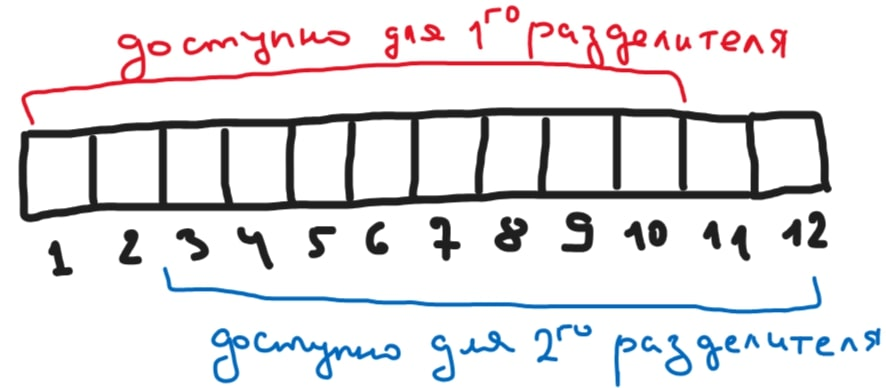
\includegraphics[width=0.5\textwidth]{pictures/HappyTicketsFor10.jpg}
\end{figure}

Итого,
\[
N(10) = 1 \cdot 9 + 1 \cdot 10 + \frac{8 \cdot 7}{2} + 8 \cdot 2 = 63.
\]

Аналогично вычисляются $N(11), N(12), N(13)$.

И тогда можно выписать таблицу:\\

\begin{center}
    \begin{tabular}{|*{15}{c|}} % 15 столбцов
    \hline
    \multicolumn{15}{|c|}{\textbf{Результаты вычислений}} \\
    \hline
    k & 0 & 1 & 2 & 3 & 4 & 5 & 6 & 7 & 8 & 9 & 10 &
    11 & 12 & 13 \\
    \hline
    N(k) & 1 & 3 & 6 & 10 & 15 & 21 & 28 & 36 & 45 &
    55 & 63 & 69 & 73 & 75\\
    \hline
    \end{tabular}
\end{center}

Остается просто просуммировать
\[
\sum_{k=0}^{27} N(k)^2 = 55252,
\]
а тогда вероятность получить счастливый билет равна
\[
\frac{55252}{1000000} = 0.055252,
\]
то есть примерно каждый 18-ый билет будет счастливым.

\threestars

Задачу можно считать решенной, все же выглядит это решение достаточно кустарно. Есть более красивые методы, рассмотрим сначала идею из \cite{OneMoreTimeAboutHappyTickets}.



\newpage
\nocite{*}
\printbibliography[nottype=unpublished]

\end{document}